% !BIB TS-program = biber

\RequirePackage[l2tabu,orthodox]{nag}

% TODO: decide if one-sided/two-sided
%\documentclass[headsepline,footsepline,footinclude=false,fontsize=11pt,paper=a4,listof=totoc,bibliography=totoc,BCOR=12mm,DIV=12]{scrbook} % two-sided
\documentclass[headsepline,footsepline,footinclude=false,oneside,fontsize=11pt,paper=a4,listof=totoc,bibliography=totoc]{scrbook} % one-sided

% TODO: change citation style in settings
\PassOptionsToPackage{table,svgnames,dvipsnames}{xcolor}

\usepackage[utf8]{inputenc}
\usepackage[T1]{fontenc}
\usepackage[sc]{mathpazo}
\usepackage[ngerman,american]{babel}
\usepackage[autostyle]{csquotes}
\usepackage[%
  backend=biber,
  url=true,
  style=authoryear,
  maxnames=4,
  minnames=3,
  maxbibnames=99,
  giveninits,
  uniquename=init]{biblatex} % TODO: adapt citation style
\usepackage{graphicx}
\usepackage{svg}
\usepackage{amsfonts}
\usepackage{bm}
\usepackage{physics}
\usepackage{algorithm}
\usepackage[noEnd=true, indLines=false]{algpseudocodex}
\algrenewcommand{\algorithmicforall}{\textbf{for each}}
\newcommand{\algorithmautorefname}{Algorithm}
\usepackage{scrhack} % necessary for listings package
\usepackage{listings}
\usepackage{lstautogobble}
\usepackage{tikz}
\usetikzlibrary{external}
\tikzexternalize[prefix=tikzfigures/]
\usepackage{pgfplots}
\usepackage{pgfplotstable}
\usepackage{booktabs}
\usepackage[final]{microtype}
\usepackage{caption}
\usepackage[printonlyused]{acronym}
\usepackage[hidelinks]{hyperref} % hidelinks removes colored boxes around references and links
\AtBeginDocument{%
	\hypersetup{
		pdftitle=\getTitle,
		pdfauthor=\getAuthor,
	}
}
\usepackage{ifthen}

% for fachschaft_print.pdf
\makeatletter
\if@twoside
	\typeout{TUM-Dev LaTeX-Thesis-Template: twoside}
\else
	\typeout{TUM-Dev LaTeX-Thesis-Template: oneside}
\fi
\makeatother

\addto\extrasamerican{
	\def\lstnumberautorefname{Line}
	\def\chapterautorefname{Chapter}
	\def\sectionautorefname{Section}
	\def\subsectionautorefname{Subsection}
	\def\subsubsectionautorefname{Subsubsection}
}

\addto\extrasngerman{
	\def\lstnumberautorefname{Zeile}
}

% Themes
\ifthenelse{\equal{\detokenize{dark}}{\jobname}}{%
  % Dark theme
  \newcommand{\bg}{black} % background
  \newcommand{\fg}{white} % foreground
  \usepackage[pagecolor=\bg]{pagecolor}
  \color{\fg}
}{%
  % Light theme
  \newcommand{\bg}{white} % background
  \newcommand{\fg}{black} % foreground
}

\bibliography{bibliography}

\setkomafont{disposition}{\normalfont\bfseries} % use serif font for headings
\linespread{1.05} % adjust line spread for mathpazo font

% Add table of contents to PDF bookmarks
\BeforeTOCHead[toc]{{\cleardoublepage\pdfbookmark[0]{\contentsname}{toc}}}

% Define TUM corporate design colors
% Taken from http://portal.mytum.de/corporatedesign/index_print/vorlagen/index_farben
\definecolor{TUMBlue}{HTML}{0065BD}
\definecolor{TUMSecondaryBlue}{HTML}{005293}
\definecolor{TUMSecondaryBlue2}{HTML}{003359}
\definecolor{TUMBlack}{HTML}{000000}
\definecolor{TUMWhite}{HTML}{FFFFFF}
\definecolor{TUMDarkGray}{HTML}{333333}
\definecolor{TUMGray}{HTML}{808080}
\definecolor{TUMLightGray}{HTML}{CCCCC6}
\definecolor{TUMAccentGray}{HTML}{DAD7CB}
\definecolor{TUMAccentOrange}{HTML}{E37222}
\definecolor{TUMAccentGreen}{HTML}{A2AD00}
\definecolor{TUMAccentLightBlue}{HTML}{98C6EA}
\definecolor{TUMAccentBlue}{HTML}{64A0C8}

% Settings for pgfplots
\pgfplotsset{compat=newest}
\pgfplotsset{
  % For available color names, see http://www.latextemplates.com/svgnames-colors
  cycle list={TUMBlue\\TUMAccentOrange\\TUMAccentGreen\\TUMSecondaryBlue2\\TUMDarkGray\\},
}

% Settings for lstlistings
\lstset{%
  basicstyle=\ttfamily,
  columns=fullflexible,
  autogobble,
  keywordstyle=\bfseries\color{TUMBlue},
  stringstyle=\color{TUMAccentGreen},
  captionpos=b
}


% TODO: change thesis information
\newcommand*{\getUniversity}{Technische Universität München}
\newcommand*{\getFaculty}{Informatics}
\newcommand*{\getDegree}{Informatics}
\newcommand*{\getSchool}{Computation, Information and Technology}
\newcommand*{\getTitle}{Gradientless Optimization for Language Model Finetuning}
\newcommand*{\getTitleGer}{Gradientenfreie Optimierung für Language Model Finetuning}
\newcommand*{\getAuthor}{Cosku Baris Coslu}
\newcommand*{\getDoctype}{Master's Thesis}
\newcommand*{\getSupervisor}{Prof. Dr. Georg Groh}
\newcommand*{\getAdvisor}{Jeremias Bohn}
\newcommand*{\getSubmissionDate}{15.07.2024}
\newcommand*{\getSubmissionLocation}{Munich}

\begin{document}

% Set page numbering to avoid "destination with the same identifier has been already used" warning for cover page.
% (see https://en.wikibooks.org/wiki/LaTeX/Hyperlinks#Problems_with_Links_and_Pages).
\pagenumbering{alph}
\begin{titlepage}
  % HACK for two-sided documents: ignore binding correction for cover page.
  % Adapted from Markus Kohm's KOMA-Script titlepage=firstiscover handling.
  % See http://mirrors.ctan.org/macros/latex/contrib/koma-script/scrkernel-title.dtx,
  % \maketitle macro.
  \oddsidemargin=\evensidemargin\relax
  \textwidth=\dimexpr\paperwidth-2\evensidemargin-2in\relax
  \hsize=\textwidth\relax

  \centering

  \IfFileExists{logos/tum-\fg.pdf}{%
    \includegraphics[height=20mm]{logos/tum-\fg.pdf}
  }{%
    \vspace*{20mm}
  }

  \vspace{5mm}
  {\huge\MakeUppercase{School of \getSchool{} --- \getFaculty{}} \par}

  \vspace{5mm}
  {\large\MakeUppercase{\getUniversity{}} \par}

  \vspace{15mm}
  {\Large \getDoctype{} in \getDegree{} \par}

  \vspace{10mm}
  {\huge\bfseries \getTitle{} \par}

  \vspace{10mm}
  {\LARGE \getAuthor{}}

  \IfFileExists{logos/faculty-\fg.pdf}{%
    \vfill{}
    \includegraphics[height=20mm]{logos/faculty-\fg.pdf}
  }{}
\end{titlepage}


\frontmatter{}

\begin{titlepage}
  \centering

  \IfFileExists{logos/tum-\fg.pdf}{%
    \includegraphics[height=20mm]{logos/tum-\fg.pdf}
  }{%
    \vspace*{20mm}
  }

  \vspace{5mm}
  {\huge\MakeUppercase{School of \getSchool{} --- \getFaculty{}} \par}

  \vspace{5mm}
  {\large\MakeUppercase{\getUniversity{}} \par}

  \vspace{20mm}
  {\Large \getDoctype{} in \getDegree{} \par}

  \vspace{15mm}
  {\huge\bfseries \getTitle{} \par}

  \vspace{10mm}
  {\huge\bfseries \foreignlanguage{ngerman}{\getTitleGer{}} \par}

  \vspace{15mm}
  \begin{tabular}{l l}
    Author:          & \getAuthor{}         \\
    Supervisor:      & \getSupervisor{}     \\
    Advisor:         & \getAdvisor{}        \\
    Submission Date: & \getSubmissionDate{} \\
  \end{tabular}

  \IfFileExists{logos/faculty-\fg.pdf}{%
    \vfill{}
    \includegraphics[height=20mm]{logos/faculty-\fg.pdf}
  }{}
\end{titlepage}

\thispagestyle{empty}
\vspace*{0.8\textheight}
\noindent
I confirm that this \MakeLowercase{\getDoctype{}} is my own work and I have documented all sources and material used.

\vspace{15mm}
\noindent
\getSubmissionLocation{}, \getSubmissionDate{} \hspace{\fill} \getAuthor{}

\cleardoublepage{}

% \addcontentsline{toc}{chapter}{Acknowledgments}
\thispagestyle{empty}

\vspace*{20mm}

\begin{center}
    {\usekomafont{sectioning}\usekomafont{section} Acknowledgments}
\end{center}

\vspace{10mm}

%TODO: Acknowledgments

\cleardoublepage{}

\chapter{\abstractname}

Transformer models pre-trained on large amounts of data 
have become the standard method of building powerful
language models in \ac{NLP} research. These models 
incorporate comprehensive information about language, 
allowing them to be fine-tuned for a wide variety 
of tasks using a smaller, task-specific dataset
without substantial modifications on the architecture. 
This work aims to explore gradientless optimization 
methods that can be utilized in the context of language 
model fine-tuning. In particular, it investigates
the feasibility 
of using direct search methods 
based on random perturbations of parameter tensors 
as an alternative 
to state-of-the-art first-order optimizers for the 
fine-tuning of pre-trained language models. 
We introduce a direct search 
method based on an adaptation of the \ac{GLD} algorithm. 
Our method can 
fine-tune a DistilBERT model on the SST-2 dataset 
using less memory than an Adam optimizer in exchange 
for a small reduction in validation accuracy.

\microtypesetup{protrusion=false}
\tableofcontents{}
\microtypesetup{protrusion=true}

\mainmatter{}

\chapter{Introduction}\label{chapter:introduction}

Neural Networks are powerful machine 
learning models that have been shown to 
yield state-of-the-art results 
in the field of \acf{NLP} \parencite{goldberg2016primer}.
Recently, the Transformer \parencite{transformer}
has been adopted as a conventional architecture for 
creating language models. Transformer models such as 
BERT \parencite{bert} have been shown to learn 
comprehensive information about language when trained on 
unsupervised language modeling tasks with 
large amounts of data. Representations
learned by these models are useful for a wide variety of 
tasks and the same pre-trained model can be fine-tuned 
for different tasks by adding an appropriate output layer
and training it on a smaller, task-specific dataset. 

A neural network model is trained by iteratively updating
its parameters in order to minimize a 
loss function measuring the error between 
observed data and the model output. 
The standard method of training
relies on the backpropagation algorithm 
\parencite{backprop} to calculate the gradient 
of the loss function w.r.t the parameters 
of the model. The gradient is used to find the descent 
direction and parameters are moved in that
direction to minimize the loss. 

In general, optimization algorithms that make use of 
the gradient are called first-order methods referring
to the order of the used derivatives. 
There are also zeroth-order
methods that only need to evaluate a function at 
different points in order to optimize it. Zeroth-order
methods have proven to be useful in generating
adversarial examples for machine learning 
systems \parencite{adversarial} as well as in 
automated machine learning research \parencite{automl}.
They can also be used when gradient calculation 
is infeasible or impractical \parencite{primer-zo}. 

Many zeroth-order
methods such as ZO-SGD \parencite{spsa}, 
ZO-AdaMM \parencite{zoadamm} and MeZO \parencite{mezo}
calculate an estimation of the gradient using 
finite difference approximations, which can then be used
in the place of the gradient. As such, these algorithms 
are easily implemented by only slightly modifying 
common first-order methods \parencite{primer-zo}. 
Other zeroth-order algorithms, such as 
\ac{STP} \parencite{stp} and \acf{GLD} \parencite{gld}, 
perform a search in a small radius around a parameter 
and update it to the best candidate. 
Algorithms from this class are called direct search 
methods. 
Direct search methods are not often used for the purpose
of training neural networks as they do not scale well 
to large-size problems \parencite{directsearch}. 

Training large neural networks can be costly 
in terms of memory. 
Reducing the memory usage can be beneficial to make 
research more accessible by making neural network training 
possible on systems with limited computational resources.
Recent approaches reduce the model size by pruning
neurons from the network \parencite{pruning}, 
train smaller models with the help of larger pre-trained 
models using knowledge distillation \parencite{distillation}
or reduce the memory usage of fine-tuning by training only 
a small subset of parameters \parencite{peft}. 

This work
aims to reduce the memory consumption of fine-tuning 
by using a gradientless optimization method, eliminating 
the need for backpropagation. In doing so, 
we also want to investigate the potential of 
direct search methods to train neural networks. We 
introduce an algorithm based on \ac{GLD} that can 
effectively bypass the limitations of direct search methods 
on problem size. Using
our algorithm, we fine-tune a feed-forward network 
attached to a pre-trained DistilBERT 
model \parencite{distilbert} on the SST-2 dataset 
\parencite{sst2} and obtain 
a validation accuracy comparable to that of an 
Adam optimizer \parencite{adam} while using less memory.

% Recently there has been 
% a growing interest in reducing the size of neural
% network models in order to make training possible
% on systems with limited computational resources



\chapter{Background}\label{chapter:background}
The field of \ac{NLP} comprises various computational tasks 
involving human language, such as language modeling, 
machine translation, sentiment classification
and question answering. Current state-of-the-art results 
in the field are predominantly 
produced by neural network models \parencite{goldberg2016primer}.
This chapter provides the basic background for neural networks, 
introduces several neural network architectures with 
a focus on their utilization in \ac{NLP}, surveys various 
gradient-based and gradient-free approaches to optimization 
and examines methods to rank network parameters on importance.

\section{Neural Networks} \label{section:neuralnetworks}
Neural networks are a collection of powerful machine learning tools
that see persistent use in \ac{NLP} 
and yield many of the 
recent state-of-the-art results in the field. The concept of the 
neural network takes inspiration from the human nervous system:
It models a network of basic computation units, called \textit{neurons}, 
which are connected with each other in specific layouts
similarly to the nerve cells in the brain \parencite[Chapter 1.2]{neuronbook}. 
In particular, the concept 
originates from the McCulloch–Pitts Neuron \parencite{mcculloch},
% also known as the \textit{perceptron},
which, slightly modified, is commonly used up to present \parencite{perceptronbook}.
% which models the neuron as a node that applies a linear 
% transformation on its inputs to generate a single output. 
% which models the neuron as a node that processes the inputs of
% all incoming connections from other nodes into a single output.
% In a modern neural network, 
% Each of the neuron's inputs has an associated weight. The neuron 
% sums each of its inputs multiplied by its weight and applies
% a transfer function called the \textit{activation function}
% to generate the output. 

\subsection{The Neuron}
A neuron in a neural network is a node that processes inputs 
from all incoming connections into a single output. 
Each of a neuron's inputs has an associated weight. 
The output is computed by taking the sum of all inputs
multiplied by their weights, adding a bias term and applying
a nonlinear \textit{activation function} on the sum. 
Precisely, a neuron with \(n\) incoming connections (\(n\) 
inputs, which can be expressed as a row vector \(x \in \mathbb{R}^{1\times n}\)),
computes 
% The neuron
% sums each of its inputs multiplied by its weight and adds a bias term.
% It then applies a nonlinear \textit{activation function} to this sum

% to generate its output. It computes:
\begin{equation}
    y = \sigma(\mathbf{x}\mathbf{w} + b)
\end{equation}
where \(\mathbf{w} \in \mathbb{R}^n\) is the vector of weights, 
\(b \in \mathbb{R}\) is the bias term and 
\(\sigma: \mathbb{R} \rightarrow \mathbb{R}\) is the nonlinear activation
function. \autoref{figure:neuron} visualizes a neuron in the 
form of a computation graph.

\begin{figure}
    \centering
    \includesvg[width=0.7\textwidth]{figures/neuron}
    \caption{Computation graph of a neuron}
    \label{figure:neuron}
\end{figure}

The nonlinearity from the activation function is crucial 
for the computational power of the neural network, since without 
it, the network can only represent linear transformations of
the input. Common activation 
functions are the sigmoid function,
\[\sigma(x)=\frac{1}{1+e^{-x}}\]
the hyperbolic tangent (tanh) function 
\[\textrm{tanh}(x)= \frac{e^{2x}-1}{e^{2x} + 1}\] and 
the \ac{ReLU} function
\[\textrm{ReLU}(x) = max(0, x)\].

The choice of activation function is usually made empirically and 
it has been established that in general, the ReLU function 
works better in neural networks than the presented alternatives \parencite{goldberg2016primer}.

In the following, we will discuss key neural network
architectures and their use-cases in \ac{NLP}.

\subsection{Feed-Forward Neural Networks}
The simplest kind of neural network is the 
feed-forward network, where nodes are 
connected with no cycles \parencite{jurafsky}. A feed-forward network
is usually arranged in layers: A layer for the inputs, 
a layer for the outputs and one or more \textit{hidden layers} of 
neurons in between. Connections are in one direction, where 
the outputs from units in each layer are passed to 
units in the next higher layer and there are no connections 
between units of the same layer. A special case is the 
\textit{fully-connected} feed-forward network, where each node
is connected to all nodes of the next layer. 
\autoref{figure:feedforward} shows an example of a fully-connected
network with a single hidden layer. The visualized network 
performs two linear transformations: First, the input is transformed 
from 3 dimensions to 4 dimensions, then the result is transformed 
from 4 dimensions to 2 dimensions. The calculation performed by the 
network can be expressed concisely in the form of matrix-vector 
operations:
\begin{equation} \label{equation:feedforward}
    y = \sigma(\mathbf{x}\mathbf{W_1} + \mathbf{b_1})\mathbf{W_2} + \mathbf{b_2}
\end{equation}
where \(\mathbf{x} \in \mathbb{R}^{1 \times 3}\) is the input,
\(\mathbf{W_1} \in \mathbb{R}^{3 \times 4}; 
\mathbf{b_1} \in \mathbb{R}^{1 \times 4};
\mathbf{W_2} \in \mathbb{R}^{4 \times 2}; 
\mathbf{b_2} \in \mathbb{R}^{1 \times 2}\) are the weights and 
biases for the first and the second linear transformations 
respectively, and 
\(\sigma: \mathbb{R}^{1 \times 4}\rightarrow \mathbb{R}^{1 \times 4}\)
is the nonlinearity of the hidden layer.

\begin{figure}
    \centering
    \includesvg{figures/feedforward}
    \caption[Example of a fully-connected feed-forward network]{An example of a fully-connected feed-forward network
    with a single hidden layer. The network takes 
    a 3 dimensional input and produces a 2 dimensional output. Nodes 
    in the hidden layer apply a nonlinear activation function to 
    their outputs.}
    \label{figure:feedforward}
\end{figure}

\subsection{Neural Network Training} \label{section:training}
In order to fulfill a given task, a neural network needs
to be trained on a dataset. The purpose of training is to find
the ideal set of parameters (weights and biases) 
that best align the model with the 
observed data. We are interested in the 
\textit{supervised learning} setting, where the dataset
contains pairs \((x_i, y_i)\) of input and output and the model
is supposed to learn an underlying function of the data 
such that it produces output \(y_i\) given input \(x_i\).
This involves solving an optimization problem
\begin{equation}
    \min_{\bm{\theta}} \mathcal{J}(\bm{\theta}; \mathbf{x}, \mathbf{y})
\end{equation}
where $\bm{\theta}$ are the model parameters, $\mathbf{x}$ and
$\mathbf{y}$ are inputs and outputs from the dataset, 
and $\mathcal{J}$ is 
called the \textit{objective function}. 
The goal of training is to find 
the parameters $\bm{\theta}$ that minimize the objective function. 
Different approaches to solve this optimization problem 
will be examined in \autoref{section:optimization}.

Intuitively, $\mathcal{J}$ is a function that 
calculates the output $\mathbf{\hat{y}}$ of the model 
parameterized by $\bm{\theta}$
for the given inputs $\mathbf{x}$ and
measures the error between 
the model output and the observed data.
This error is also called \textit{loss} and can be calculated 
using a loss function. 
% where the goal is to minimize the \textit{loss} function,
% a function measuring the error between 
% the model and the observed data. The optimization 
% problem, as well as different approaches to solve it, 
% will be examined in \autoref{section:optimization}.
Given true output (or \textit{label}) \(\mathbf{y}\) 
and model output \(\mathbf{\hat{y}}\), a loss function $\mathcal{L}$
returns a scalar value for error. 
The objective of training is then minimizing the loss function
\begin{equation}
    \mathcal{J}(\bm{\theta}; \mathbf{x}, \mathbf{y}) = \mathcal{L}(\mathbf{\hat{y}}, \mathbf{y})
\end{equation}
The choice of loss function 
depends mainly on the task and the outputs expected from the 
model. For example, usually, the \textit{cross-entropy} loss is used 
for classification tasks where the output 
is supposed to be interpreted as a probability distribution 
over \(k\) classes:
\begin{equation}\label{equation:crossentropy}
    \mathcal{L}_{cross-entropy}(\mathbf{\hat{y}}, \mathbf{y}) = -\sum_{i=1}^{k} y_i\log{(\hat{y}_i)}
\end{equation}
For so-called hard classification tasks where 
the label vector \(\mathbf{y}\) contains a 1 for the correct class assignment $t$
and 0 for every other class assignment, \autoref{equation:crossentropy} 
simplifies to
\begin{equation}
    \mathcal{L}_{cross-entropy}(\mathbf{\hat{y}}, \mathbf{y}) = -\log{(\hat{y}_t)}
\end{equation}
Typically, the model is trained for a certain number of iterations, 
where in each step loss is calculated and parameters are 
updated according to a certain optimization algorithm.

While training optimizes network parameters to align model
outputs to observed data, a model is only good if it can 
also perform well on previously unobserved data. The ability of a model
to perform well on unseen data is called 
\textit{generalization} and is a central challenge in 
machine learning \Parencite[Chapter 5]{deeplearningbook}.
% To ensure that the model generalizes well, a part of the 
% dataset is split and is not used for the training algorithm. 
% Instead, loss is calculated on that split regularly to 
% have an estimation on the model's ability to generalize.
% To ensure that the model generalizes well, a part of the 
% dataset is split. The split part is called the \textit{validation dataset}
% and unlike the \textit{training dataset}, is not used for the 
% training algorithm. Instead, loss is calculated on 
% the validation dataset regularly to 
% have an estimation on the model's ability to generalize.
% To ensure that the model generalizes well, the dataset is split
% into parts for training and validation. The training algorithm
% runs as usual on the \textit{training dataset}, whereas the 
% \textit{validation dataset} is not used to optimize parameters.
% Instead, loss is calculated on the validation dataset regularly 
% to have an estimation on the model's ability to generalize. 
A model's ability to generalize is measured by
calculating loss on a subset of the available data called the 
\textit{validation dataset}. This loss
is not used to optimize the parameters, but as an estimate 
on how well the model generalizes. The subset used to train
the model parameters is then called the \textit{training dataset}. 
% The examples in each dataset need to be independent from each 
% other and the both datasets need to be identically distributed. 

A common issue when training a neural network model
is \textit{overfitting}, where the model 
performs well on the training dataset but does not generalize.
One can discern that the model is overfitting when
validation loss is high with a large difference to training loss.
Typically, validation loss decreases together with training loss
at the beginning of training. While training loss keeps decreasing 
as it approaches the minimum possible loss value, validation loss
begins rising after a certain number of iterations as the model
begins to fit the noise in the data rather than the underlying 
function, hurting its generalization \parencite[Chapter 2.2]{neuronbook}. 
Thus, a simple way to ensure generalization is to stop training
when validation loss begins to rise and take the model parameters
from the iteration with the lowest validation loss.

The occurrence of overfitting is tightly connected to 
\textit{capacity}, a model's 
ability to fit a wide variety of functions, i.e. how much a model
can learn. For neural networks, capacity depends largely on
the number of parameters and the number of output components
\parencite{capacity}. That means capacity can be increased by 
adding more layers or neurons to the network architecture. 
When capacity is too large, the model 
learns the noise in the data and overfitting occurs. 
Conversely, when capacity is too small, \textit{underfitting}
may occur, which means  the model cannot perform well 
on the training dataset. Ideally, model capacity is 
adapted such that neither overfitting nor underfitting occur. 

% Other factors that affect the 
% generalization capability are the size of the training dataset 
% and the complexity of the problem. 

One method to control a model's capacity without changing 
its architecture is to implement \textit{regularization}. 
% To be more precise, 
Regularization is the common name of strategies that 
modify the training algorithm with the intention of reducing
validation loss, possibly at the expense of increased training 
loss \Parencite[Chapter 5]{deeplearningbook}. 
Usually, a penalty term on the parameters 
called the regularizer is added to 
the objective function, meaning the training algorithm
optimizes the  (weighted) sum of loss and regularizer:
\begin{equation}
    \mathcal{J}(\bm{\theta}; \mathbf{x}, \mathbf{y}) = \mathcal{L}(\mathbf{\hat{y}}, \mathbf{y}) + \lambda \cdot \Omega(\bm{\theta})
\end{equation}
where $\Omega: \mathbb{R}^n \rightarrow \mathbb{R}$ is 
the regularizer term and $\lambda \in \mathbb{R}$ is its weight.
The regularizer 
can stem from specific kinds of prior knowledge on the data, 
or it can express a generic preference for one type of model 
over others.

A common regularization method is the $L_2$-regularization, 
often also called weight decay, 
where the regularizer term is the (squared)
$L_2$-norm of the parameters:
\begin{equation}
    \Omega(\bm{\theta}) = \Vert\bm{\theta}\Vert_{2}^{2} = \bm{\theta}^T\bm{\theta}
\end{equation}
$L_2$-regularization encodes a preference for smaller weights.
This helps the model's generalization under the assumption 
that the underlying function the model is supposed to learn is 
\textit{smooth}, meaning small changes in the input do not cause
large changes in the output. The weight $\lambda$ can then
be understood as balancing the trade-off between 
smoothing and minimizing the error \parencite{regularization}. 
% It usually 
% involves adding a penalty term to the training objective 
% called the regularizer, meaning the training algorithm 
% optimizes the sum of loss and regularizer
% (i.e. training optimizes the sum of loss and regularizer).     

% Then, after training for a
% certain number of iterations, validation loss begins to increase
% while training loss is still going down. This is the point where 
% overfitting occurs as the model begins to fit the noise in the data
% rather than the underlying function. 

% Conversely, there is \textit{underfitting}, where the model 
% cannot perform well on the training dataset. In this case, 
% training loss is too high. Overfitting and underfitting occur 
% largely due to suboptimal \textit{capacity}, the model's 
% ability to fit a wide variety of functions.

\subsection{Neural Networks in Natural Language Processing}
In \ac{NLP}, tasks often involve analyzing \textit{documents}, 
collections of sentences and words. A document needs to be 
turned into a vector of real numbers before being given as input to a neural network. 
For that, it needs to be segmented into core components, which can 
be words, sub-words or some specific meaningful morphemes like 
\textit{-est} or \textit{-er} \parencite[Chapter 2]{jurafsky}. Each of these components are then 
assigned a number called a \textit{token}. This process is called 
tokenization and is performed by applying a tokenizer function.

% To perform its task, 
% the neural network then has to work with 
Given tokens as input, the neural network has to extract
\textit{features} of the document relevant for the task, such as words 
and part-of-speech tags (classification of words as noun, verb, etc.).
Each such feature is represented as a vector called the 
\textit{embedding} of the feature. While embeddings can be 
retrieved externally and fed
into the network, they are often
modeled as part of the network, resulting from an 
embedding layer, meaning representations
of features are also learned during training and 
training will cause similar features to have similar vectors \parencite{goldberg2016primer}.

The output is generated by applying transformations on the 
extracted combination of features as in \autoref{equation:feedforward}.
Depending on the task, the network may also
perform an output transformation. For example, for classification
tasks, the softmax function is applied, which transforms the 
\(k\)-dimensional output
into a probability distribution over \(k\) classes:

\begin{equation}
    \textrm{softmax}(x_i) = \frac{e^{x_i}}{\sum_{j=1}^{k}e^{x_j}}
\end{equation}

% Thus, the neural network is given tokens as input, for which 
% it extracts embeddings from its embedding layer. Then, 
% having learned the optimal weights and biases during training,
% it performs a number of transformations on the features to
% generate an output. Depending on the task, it also often
% performs an output transformation. 

% In \ac{NLP}, tasks often involve analyzing \textit{documents}, 
% collections of sentences and words. The input to a neural network
% then contains \textit{features} of the document, information that 
% is useful in fulfilling the task, such as the number of words 
% in the document 
% with a positive or negative connotation for sentiment analysis. 
% Wether or not some specific word or symbol occurs in the document,
% wether some words are written in upper case or lower case, 
% or the overall word count can also be useful features, 
% depending on the task. These features can be handcrafted for
% the input set of documents with linguistic intuition, or they can 
% be created automatically using representation learning methods.

% To use such network in \ac{NLP}, the inputs, which are often 
% made of words and sentences, need to be turned into 
% fixed-size vectors. 
% These vectors are then called \textit{word embeddings}. 

% In \ac{NLP}, the inputs of a task are often words and sentences. 
% To be used as the input of They need to be turned into fixed-size vectors using a variety 
% of methods called \textit{word embeddings}. One simple 
% method is 

% \subsection{Recurrent Neural Networks}

% \subsection{Attention}
% The state-of-the-art method of training \acp{RNN}

\subsection{The Transformer Architecture}
The transformer architecture \parencite{transformer}
has established itself as a core component of 
state-of-the-art deep \ac{NLP} models. Language
representation models based on transformers such as
BERT \parencite{bert} have been shown to learn 
rich information about language which can be used to 
create state-of-the-art models for a wide range of tasks 
without task-specific modifications on the core architecture.
In fact, a BERT model pre-trained on large amounts of data
can be fine-tuned for a given task by only adding a 
feed-forward layer on top and training it with a 
smaller dataset.

The main component of the transformer is the 
\textit{attention} mechanism, a method to model 
dependencies between sequences over arbitrarily long 
distances. It has been used mainly in 
encoder-decoder architectures where 
through the two respectively-called 
parts, an input is first encoded 
into a fixed-length vector and that vector is then decoded 
into one output at a time. Such an architecture is often used
for machine translation tasks \parencite{translation} and
% When realized by \iac{RNN} where the encoder and decoder 
% parts are made of hidden states, attention provides
% a context for the decoder from a weighted sum of all 
% encoder hidden states, allowing the decoder to 
% \textit{attend to} parts of the source text relevant 
% to the output it is currently producing. 
the role of attention
is to provide a context 
for the decoder such that it can focus on, 
or \textit{attend to}, different parts 
of the source text relevant 
to the output it is currently producing. 
Essentially, 
the idea of attention is to evaluate the relevance of a
focus of attention with each item of a set of other items
by performing a series of comparisons
\parencite[Chapter 9]{jurafsky}.  
We will give the exact computation of attention on the 
example of a self-attention layer, a core component of 
a transformer block. 

Self-attention is a type of attention relating different 
positions of a single sequence. Given a sequence
of input vectors $\mathbf{x}_1, \dots, \mathbf{x}_n$,
a self-attention layer 
produces output $\mathbf{y}_1, \dots, \mathbf{y}_n$
with the same dimensionality where each 
$\mathbf{y}_i$ is the attention of the corresponding
$\mathbf{x}_i$. The relevance of two items of the 
sequence is measured by some score function. 
The simplest score function is the dot product, which 
implements relevance as similarity: 
\begin{equation}
    \textrm{score}(\mathbf{x}_i, \mathbf{x}_j) = \mathbf{x}_i \cdot \mathbf{x}_j
\end{equation}
The more similar the two vectors being compared, 
the higher the score. With $\mathbf{x}_i$ being the
focus of attention, we can compute the proportional 
relevance to each other item in the sequence using 
the softmax function:
\begin{equation}
    \alpha_{i, j} = \textrm{softmax}(\textrm{score}(\mathbf{x}_i, \mathbf{x}_j)) = \frac{\exp(\textrm{score}(\mathbf{x}_i, \mathbf{x}_j))}{\sum_{k=1}^n \exp(\textrm{score}(\mathbf{x}_i, \mathbf{x}_k))}
\end{equation} 
Attention is then computed through a weighted sum of 
all items with their proportional relevance:
\begin{equation}
    \mathbf{y}_i = \sum_{j=1}^n \alpha_{i, j} \mathbf{x}_j
\end{equation}

Each item of the sequence plays three different roles
in the above described calculation of attention:
The current focus of attention is called the 
\textit{query}. Each item is used as
a \textit{key} when being compared with the
query to calculate their proportional relevance.
Finally, each item multiplied by its relevance in the
weighted sum plays the role of a \textit{value}.
The self-attention layer of a transformer block uses 
different vectors for each of the three roles. 
The vectors are obtained
by multiplying the input with three different weight 
matrices for query, key and value:
\begin{equation}
    \mathbf{q}_i = \mathbf{W}^Q\mathbf{x}_i;\quad \mathbf{k}_i = \mathbf{W}^K\mathbf{x}_i;\quad \mathbf{v}_i = \mathbf{W}^V\mathbf{x}_i
\end{equation} 
where $\mathbf{q}_i$, $\mathbf{k}_i$ and $\mathbf{v}_i$
are query, key and value vectors respectively and 
$\mathbf{W}^Q$, $\mathbf{W}^K$ and $\mathbf{W}^V$ 
are trainable weight matrices of the layer.

The self-attention layer also divides the dot product 
attention by $\sqrt{d}$ where $d$ is the dimensionality 
of the query and key vectors. \textcite{transformer}
introduce this scaling factor to counteract the issue
of extremely small gradients of the softmax function,
which occurs when 
the dot product becomes too large as dimensionality 
grows. With that, attention is computed as: 
% With that, the self-attention layer computes
% attention as: 
\begin{equation}
    \mathbf{y}_i = \sum_{j=1}^n \textrm{softmax}\left(\frac{\mathbf{q}_i \cdot \mathbf{k}_j}{\sqrt{d}}\right) \mathbf{v}_j
\end{equation}
% \begin{equation}
%     \textrm{score}(\mathbf{x}_i, \mathbf{x}_j) = \mathbf{q}_i \cdot \mathbf{k}_j
% \end{equation}
% \begin{equation}
%     \alpha_{i, j} = \textrm{softmax}(\textrm{score}(\mathbf{x}_i, \mathbf{x}_j))
% \end{equation} 
% \begin{equation}
%     \mathbf{y}_i = \sum_{j=1}^n \alpha_{i, j} \mathbf{v}_j
% \end{equation}
In practice, attention is computed simultaneously for
a set of queries, keys and values packed together
into matrices:
\begin{equation}
    \mathbf{Y} = \textrm{softmax}\left(\frac{\mathbf{QK}^T}{\sqrt{d}}\right)\mathbf{V}
\end{equation}
A transformer block employs a so-called multi-head
attention, which is a set of self-attention layers 
that compute their outputs in parallel, each of them using
their own weight matrices. Each parallel computing unit
is called a head and can capture different types of 
relation between the inputs. The output of each head is
concatenated and projected into the 
original output dimensions 
through a final linear transformation.

The multi-head self-attention mechanism is one of the 
two main components of a transformer block. The other is 
a simple fully-connected feed-forward network.
\autoref{figure:transformer} shows the structure of a 
transformer block. There are
\textit{residual connections} around each of the two
layers, which are shortcuts that skip a layer entirely.
The input of the layer is thus added to its output 
before being passed forward in the network.
Residual connections give
higher level layers direct access to 
information from lower layers, which has been shown 
to improve the learning of deep networks
\parencite{residual}. 
Finally, the outputs are normalized, which involves
subtracting the mean and dividing by the standard
deviation, resulting in a vector of 0 mean and a 
standard deviation of 1. The normalized output
vector is then 
further transformed with a learnable weight and bias. 
This process is called \textit{layer normalization} and
has been shown to reduce the training time of deep 
networks by keeping the values of layer outputs in 
a reasonable range that gives useful gradients
\parencite{layernorm}.

% \autoref{figure:transformer} shows the structure of a 
% transformer block. Transformer networks are made of 
% stacks of those blocks. The original transformer work
% defines an encoder-decoder architecture where this
% block is the encoder. For the decoder they create 
% a slightly modified block that also employs
% encoder-decoder attention. 
% Finally, the outputs are normalized, 
% by subtracting the mean and dividing by the standard
% deviation, resulting in a vector of 0 mean and a 
% standard deviation of 1. The normalized vector is then 
% further transformed with a learnable weight and bias. 
% and pass the input of the layer forward in the network.
% The input is then added to the output 


\begin{figure}
    \centering
    \includesvg[height=0.6\textheight]{figures/transformer}
    \caption[The structure of a transformer block]
    {The structure of a transformer block. The key 
    components are a multi-head self-attention layer 
    and a feed-forward layer. There are residual 
    connections around each layer and layer normalization
    is applied on the outputs.}
    \label{figure:transformer}
\end{figure}


% The main idea of the described attention mechanism is
% to compute the relevance of the current decoder hidden 
% state with each encoder hidden state. 
% In such architecture, the encoder 
% and decoder would be \acp{RNN} and attention would be 
% utilized to 


\section{Optimization} \label{section:optimization}
% In order to fulfill the given task, a neural network needs
% to be trained. Training involves finding 
% the ideal set of trainable
% parameters w.r.t. an objective function, which, 
% in turn, means solving an optimization problem.
% In general, we are interested in solving an 
% unconstrained minimization problem,
% where the goal is to obtain the set of parameters
%  that minimize
% the \textit{loss} function, a function measuring the error between the model and the observed data. 
% The problem is 

% Given a loss function \(f: \mathbb{R}^n \rightarrow \mathbb{R}\),
In \autoref{section:training} we have established that training 
a neural network involves minimizing an objective function. This 
section is dedicated to algorithms that can solve the optimization
problem in the context of neural network training.   
In particular, we are interested in solving the following unconstrained minimization problem:
\begin{equation}
    \min_{\bm{\theta} \in \mathbb{R}^n} \mathcal{J}(\bm{\theta})
\end{equation}
where \(\mathcal{J}: \mathbb{R}^n \rightarrow \mathbb{R}\) 
is the objective function and \(\bm{\theta} \in \mathbb{R}^n\) 
contains the trainable parameters of the model.
The optimization algorithms we will introduce define 
suitable parameter updates, meaning for a 
given parameter configuration $\bm{\theta}_t$ 
at iteration $t$, they
define $\bm{\theta}_{t+1}$ with the intention of minimizing 
$\mathcal{J}$.

We will present first-order and zeroth-order methods 
of optimization, where \textit{order} refers to the 
order of the associated derivatives. Zeroth-order methods 
use only function values $\mathcal{J}(\bm{\theta})$ while 
first-order methods also make use of the gradient 
$\nabla_{\bm{\theta}} \mathcal{J}(\bm{\theta})$
\parencite{directsearch}. 

\subsection{Stochastic Gradient Descent} \label{section:sgd}
The \ac{SGD} algorithm computes the gradient
$\nabla_{\bm{\theta}} \mathcal{J}(\bm{\theta})$ at each 
step to find the right direction for $\bm{\theta}$ to
move (the descent direction). With 
$\bm{\theta} \in \mathbb{R}^n$ being the vector of parameters, 
the gradient $\nabla_{\bm{\theta}} \mathcal{J}(\bm{\theta})$
is defined as the vector of partial derivatives of 
$\mathcal{J}$ w.r.t each parameter: 
\begin{equation}
    \nabla_{\bm{\theta}} \mathcal{J}(\bm{\theta}) = 
    \begin{bmatrix}
        \pdv{\mathcal{J}}{\bm{\theta}_1}\\
        \vdots\\
        \pdv{\mathcal{J}}{\bm{\theta}_n}
    \end{bmatrix}
\end{equation}
That means finding the descent direction requires the 
partial derivative of $\mathcal{J}$ w.r.t each 
weight and bias of the network in each layer. The partial
derivatives are calculated using the chain rule of 
differentiation, which specifies the derivative of
function compositions. The derivative of a composite function 
$f(x) = u(v(x))$ w.r.t $x$ is calculated using the chain 
rule as:
\begin{equation}
    \dv{f}{x} = \dv{u}{v}\cdot\dv{v}{x}
\end{equation}

At the core of gradient calculation for \ac{SGD} and 
other gradient-based optimization methods lies the
backpropagation algorithm \parencite{backprop}, which 
does a backward pass on the network after calculating 
the objective $\mathcal{J}$ to propagate the partial
derivatives backwards beginning from the last layer. 
Each layer then takes the gradients passed in from the 
next higher layer, locally computes the partial derivatives 
of $\mathcal{J}$ w.r.t each of its parameters according to
the chain rule, and finally passes the gradients necessary
for further calculations to the next lower layer. As 
shown in \autoref{section:neuralnetworks}, each layer
in a neural network performs a chain of operations on its 
input to generate its output and the entire network can be 
represented as a computation graph where each node 
contains the intermediary result of one operation.  
\autoref{figure:backprop} shows an example of such 
computation graph expanded at one hidden layer. 
A forward pass through the computation graph calculates
the model output and loss, thus the objective. A backward
pass (shown in blue) calculates partial derivatives at
each node, where the partial derivatives at the weights 
and biases (orange nodes) are used for the 
parameter update of \ac{SGD}.

\begin{figure}
    \centering
    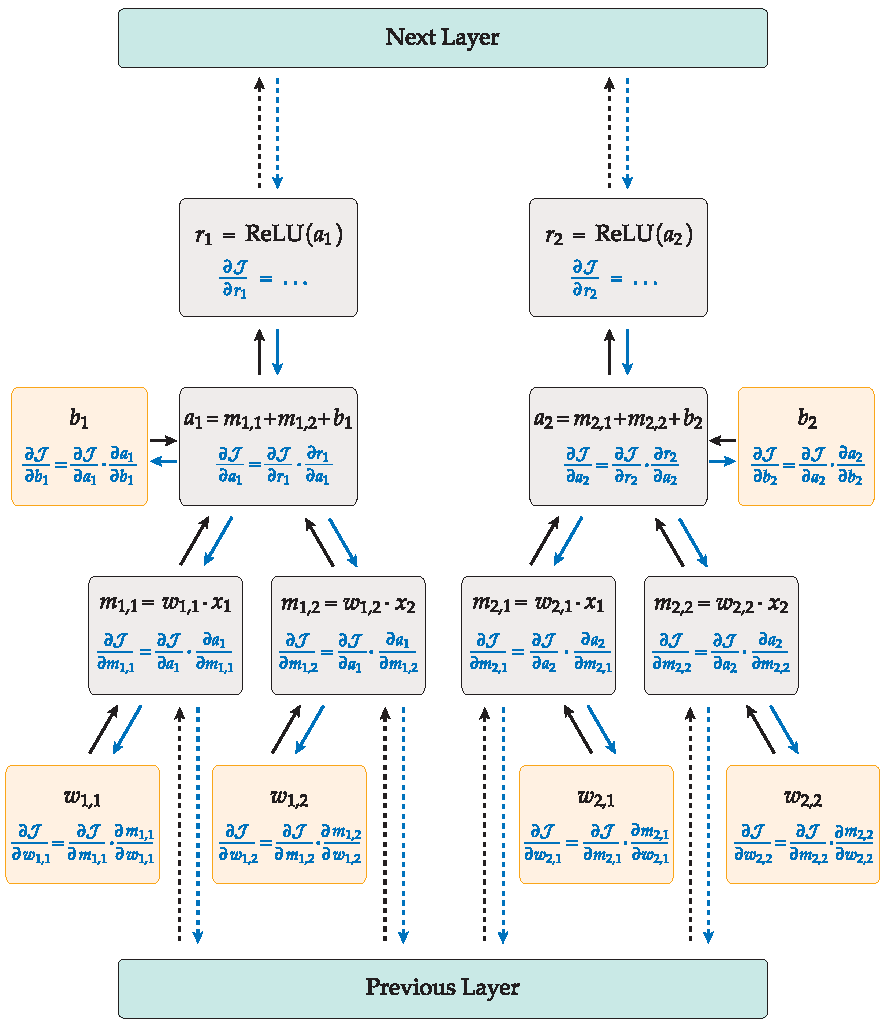
\includegraphics[height=0.85\textheight]{figures/backprop.pdf}
    \caption[Backward Pass on a Computation Graph]
    {Backward Pass on the computation graph of a 
    feed-forward network. The graph
    shows a hidden layer with two neurons. 
    The direction of the backward pass and the partial
    derivatives computed by the backpropagation algorithm
    are shown in blue. Orange nodes are the trainable 
    parameters of the layer. 
    }
    \label{figure:backprop}
\end{figure}

% locally computes the partial derivatives 
% of $\mathcal{J}$ w.r.t each of its parameters according to
% the chain rule using the gradients passed in from the higher 
% layer and finally passes the result to the next lower 
% layer.
% the backpropagation 
% algorithm \parencite{backprop}. 

Since the gradient gives the ascent direction
of the objective function, \ac{SGD} moves
 $\bm{\theta}$ in the 
opposite direction
by a certain step size $\eta$, which
is called the \textit{learning rate}. 
\autoref{equation:sgd} gives the parameter update 
of \ac{SGD}:
\begin{equation} \label{equation:sgd}
    \bm{\theta}_{t+1} = \bm{\theta}_t - \eta \cdot \nabla_{\bm{\theta}} \mathcal{J}(\bm{\theta})
\end{equation} 

The learning rate $\eta$ is a \textit{hyperparameter}
of the algorithm, meaning the choice for its value needs
to be made before applying the algorithm and plays a 
crucial role in its effectiveness: 
If the learning rate is too low, convergence to the minimum
will be too slow, whereas if it is too high, the algorithm 
might oscillate around the minimum and fail to converge. 
It can be beneficial to change the learning rate during
training such that we begin training with a larger 
learning rate to rapidly approach the minimum and 
gradually decrease the learning rate as training goes on 
to get as close to the 
minimum as possible with smaller adjustments. This can be 
achieved by using a learning rate scheduler, a function 
that returns a multiplier for $\eta$ at each step. 
The learning rate $\eta$ in \autoref{equation:sgd} can 
then be replaced by $\eta_t$, the effective learning rate
at step $t$.

\ac{SGD} is an online algorithm, which means it does not
need to process the entire input outright but can go 
through the input example by example 
\parencite[Chapter 5]{jurafsky}. Usually, inputs are
given in small groups called mini-batches:
% where the batch size is also a hyperparameter. 
In each iteration, $b$ randomly-picked samples are given as
input to the model to calculate $b$ outputs, and 
loss is averaged over the $b$ samples:
\begin{equation}
    \nabla_{\bm{\theta}} \mathcal{J}(\bm{\theta}) = 
    \frac{1}{b}\sum_{i=1}^{b}
    \nabla_{\bm{\theta}} \mathcal{J}_i(\bm{\theta})
    \;;\quad
    \mathcal{J}_i(\bm{\theta}) = \mathcal{J}(\bm{\theta}; \mathbf{x}_i, \mathbf{y}_i)
\end{equation} 
The batch size $b$ is also a hyperparameter. Smaller
batch sizes make noisy updates because of a greater 
variance in the gradients
(in the extreme case of $b=1$, parameters are updated to fit a 
single sample in each iteration). 
Larger batch sizes allow the use of larger 
learning rates while achieving the same optimal 
error bounds \parencite{minibatch} and improve
parallelism as the increased amount of computation per 
iteration can be effectively distributed. On the other hand,
they increase the memory requirement of the algorithm and  
when batch size is too high, it can 
impair the model's ability to generalize:
It has been observed that 
when using larger batch sizes, 
algorithms tend to converge 
to \textit{sharp} minimizers where the  
function increases rapidly in a small neighborhood of 
the minimum, which negatively impacts generalization 
\parencite{minibatch2}.  

\subsection{Adaptive Gradient Methods}
For efficient optimization, one needs to overcome 
a central issue of the \ac{SGD} algorithm, which is its 
slow convergence rate. As discussed in \autoref{section:sgd}, 
the convergence rate is directly bound to the learning rate $\eta$, 
but the algorithm fails to converge when $\eta$ is too high.
Thus, $\eta$ needs to be picked conservatively to avoid
divergence, resulting in excessively slow
convergence rates. Adaptive gradient methods try to solve
this issue by taking the parameter updates 
from previous iterations into account
when calculating the update 
for the current iteration. 

\subsubsection{Momentum}

Ideally, we want to take larger steps
in a direction when a sequence of previous 
gradients all pointed in that direction, effectively
accumulating gradients over time. This is the main idea
behind the momentum method \parencite{momentum-polyak}.
The momentum method calculates a velocity vector 
$\mathbf{v}$ that 
accumulates in directions that persistently reduce 
the objective function across iterations:
\begin{equation}
    \mathbf{v}_{t+1} = \beta \cdot \mathbf{v}_t - \eta \cdot \nabla_{\bm{\theta}}\mathcal{J}(\bm{\theta}_t)
\end{equation}
where $\beta \in \mathbb{R}$ is called the momentum coefficient and determines
the rate of velocity accumulation. The parameter update 
is then given using the velocity vector:
\begin{equation}
    \bm{\theta}_{t+1} = \bm{\theta}_t + \mathbf{v}_{t+1}
\end{equation}

\subsubsection{Nesterov Momentum}

Nesterov’s Accelerated Gradient, also called Nesterov 
momentum \parencite{nesterov}, is a simple modification of
the classical momentum method that has been observed to
increase stability and improve performance 
\parencite{momentum-sutskever}. Instead of computing 
the velocity using the gradient from the current
position, it first performs a partial update and uses the
gradient at the position $\bm{\theta}_t + \beta \cdot \mathbf{v}_t$:
\begin{equation}
    \mathbf{v}_{t+1} = \beta \cdot \mathbf{v}_t - \eta \cdot \nabla_{\bm{\theta}}\mathcal{J}(\bm{\theta}_t + \beta \cdot \mathbf{v}_t)
\end{equation}

\subsubsection{Adam}

The last adaptive gradient method we want to share is Adam
\parencite{adam}. Adam computes two moving averages
similar to momentum:  
\begin{equation}
    \mathbf{m}_{t+1} = \beta_1 \cdot \mathbf{m}_t + (1 - \beta_1) \cdot \nabla_{\bm{\theta}} \mathcal{J}(\bm{\theta}_{t})
\end{equation}
\begin{equation}
    \mathbf{v}_{t+1} = \beta_2 \cdot \mathbf{v}_t + (1 - \beta_2) \cdot (\nabla_{\bm{\theta}} \mathcal{J}(\bm{\theta}_{t}))^2
\end{equation}
where $\mathbf{m}$ and $\mathbf{v}$ operate as
estimates of the mean and 
the uncentered variance of the gradient respectively
and $\beta_1, \beta_2 \in [0, 1)$ control their decay rates.
$\mathbf{m}_0$ and $\mathbf{v}_0$ are initialized as 
0's, which cause a bias towards 0, especially in the 
early steps and when $\beta_1$ and $\beta_2$ are close to
1. Thus, a bias correction is applied:
\begin{equation}
    \hat{\mathbf{m}}_{t+1} = \frac{1}{1 - \beta_1^{t+1}}\mathbf{m}_{t+1}
\end{equation}
\begin{equation}
    \hat{\mathbf{v}}_{t+1} = \frac{1}{1 - \beta_2^{t+1}}\mathbf{v}_{t+1}
\end{equation}
Finally, parameters are updated using the bias-corrected 
estimates:
\begin{equation}
    \bm{\theta}_{t+1} = \bm{\theta}_t - \eta \cdot \frac{\hat{\mathbf{m}}_{t+1}}{\sqrt{\hat{\mathbf{v}}_{t+1}} + \epsilon}
\end{equation}
where $\epsilon > 0$ is a very small number. The authors 
give $\beta_1 = 0.9$, $\beta_2 = 0.999$ and 
$\epsilon = 10^{-8}$ as good default settings with
$\eta = 0.001$.

\subsection{Finite Difference Methods}
Finite difference methods are 
zeroth-order methods that solve an optimization problem
using the same recipe as first-order gradient methods, only
without explicit computation of a gradient. Instead, 
gradients are estimated from a sequence of 
function evaluations, effectively requiring only forward
passes to train a neural network.

The Kiefer-Wolfowitz finite-difference algorithm
\parencite{KieferWolfowitz} approximates the derivative 
of a function $f(x)$ as
\begin{equation}\label{equation:finitediff}
    f'(x) \approx \frac{f(x+h)-f(x-h)}{2h}
\end{equation}
The quantity $h$ is 
called the finite difference interval and using the 
Taylor series expansion, the following relation 
can be shown for
sufficiently small intervals
\parencite[Page 54]{optimizationbook2}:
\begin{equation}
    \frac{f(x+h)-f(x-h)}{2h} = f'(x) + O(h^2)
\end{equation}
Using the Kiefer-Wolfowitz finite difference, we can obtain 
a gradient approximation $\hat{\nabla}\mathcal{J}(\bm{\theta})$:
\begin{equation}
    \hat{\nabla}_i \mathcal{J}(\bm{\theta}) = \frac{\mathcal{J}(\bm{\theta} + h \cdot \mathbf{e}_i) - \mathcal{J}(\bm{\theta} - h \cdot \mathbf{e}_i)}{2h}
\end{equation} 
\begin{equation}
    \hat{\nabla} \mathcal{J}(\bm{\theta}) = (\hat{\nabla}_1 \mathcal{J}(\bm{\theta}), \hat{\nabla}_2 \mathcal{J}(\bm{\theta}), \dots, \hat{\nabla}_n \mathcal{J}(\bm{\theta}))^T
\end{equation} 
where $\mathbf{e}_i$ is the $i$-th unit vector. The disadvantage of this method is the 
large number of function evaluations it requires 
($2n$ evaluations for $n$-dimensional $\bm{\theta})$
\parencite{finitediffpaper}. 

\ac{SPSA} \parencite{spsa} reduces the number of function
evaluations to 2 by perturbing all directions at the 
same time: 
\begin{equation} \label{equation:spsa}
    \hat{\nabla} \mathcal{J}(\bm{\theta}) = \frac{\mathcal{J}(\bm{\theta} + h\cdot\mathbf{z}) - \mathcal{J}(\bm{\theta} - h\cdot\mathbf{z})}{2h} \cdot \mathbf{z}
\end{equation}
where $\mathbf{z} \in \mathbb{R}^n$ is a vector of small 
random perturbations and can be sampled, e.g.\ 
from a standard gaussian
distribution with $z_i \sim \mathcal{N}(0, 1)$.
Using the gradient estimate from \autoref{equation:spsa}
as a replacement for the gradient in \autoref{equation:sgd}
(\ac{SGD}),
we obtain the \textbf{ZO-SGD} algorithm \parencite{spsa}.

The \textbf{ZO-signSGD} algorithm \parencite{zosignsgd} 
instead uses the sign
of the estimated gradient as direction for the update.
It has been shown that the first-order signSGD 
algorithm \parencite{signsgd}
yields an empirically faster convergence speed than standard 
\ac{SGD} 
% as taking the sign of the gradient can mitigate 
% the negative effect of gradient noise of large variance. 
ZO-signSGD shows analogous improvements in 
convergence rate over ZO-SGD. However, it has worse 
convergence accuracy than ZO-SGD as it only converges 
to a neighborhood of the minimum \parencite{zoadamm}.

\textbf{MeZO} \parencite{mezo} proposes a memory-efficient 
implementation of ZO-SGD where the algorithm does not store 
the random perturbation vector 
$\mathbf{z}$ of \autoref{equation:spsa}. Instead, 
the random seed is stored and the random number generator
is reset by this seed to resample $\mathbf{z}$ for each 
of its uses, giving a
memory footprint equivalent to the inference memory cost.

The zeroth-order adaptive momentum method (\textbf{ZO-AdaMM})
\parencite{zoadamm} implements an adaptive gradient method
using the zeroth-order gradient estimate. It fuses the 
gradient estimate with AMSGrad 
\parencite{amsgrad}, which is a modified version of Adam. 
Compared to other zeroth-order methods, 
the authors show superior performance and convergence rate 
for the task of designing adversarial examples. 

% Consider the definition of the derivative 
% of a function $f(x)$: 
% \begin{equation}\label{equation:finitediff}
%     f'(x) = \lim_{h \rightarrow 0} \frac{f(x+h)-f(x)}{h}
% \end{equation}
% The difference $f(x+h) - f(x)$ of function evaluations is 
% called a finite difference and can be used to estimate 
% the gradient of $f$ at a point $x$ \parencite{optimizationbook}.
% The quantity $h$ is 
% called the finite difference interval. Instead of 
% calculating the derivative analytically as the limit, one 
% can approximate the derivative by using a 
% small finite
% difference interval. Using the Taylor series expansion, 
% \textcite[Section 2.3.5]{optimizationbook2} show the following 
% relation for sufficiently small $h$: 
% \begin{equation}
%     \frac{f(x+h)-f(x)}{h} = f'(x) + O(h) 
% \end{equation}

\subsection{Direct Search Methods} \label{section:directsearch}
% Under direct search methods we will present zeroth-order 
% methods that do not use an approximation of the gradient.
Unlike the previously discussed finite difference 
methods, direct search methods do not rely on a 
gradient approximation.
Instead, they conduct a search by identifying 
possible candidates $\bm{\hat{\theta}}_1, \dots \bm{\hat{\theta}}_c$, 
for the parameter vector $\bm{\theta}$, 
evaluating the objective function $\mathcal{J}$ 
on those points and updating the parameters 
to the best candidate: 
\begin{equation}
    \bm{\theta}_{t+1} = \arg\min_{\bm{\hat{\theta}}} \{\mathcal{J}(\bm{\hat{\theta}}) | \bm{\hat{\theta}} \in \{\bm{\hat{\theta}}_1, \dots, \bm{\hat{\theta}}_c\}\}
\end{equation}
Typically, a candidate
is determined by adding a random perturbation vector to
the current parameter: 
\begin{equation}
    \bm{\hat{\theta}}_k = \bm{\theta}_t + \mathbf{z}_k \;;\quad \mathbf{z}_k \sim \mathcal{D}_k 
\end{equation}
where $\mathcal{D}_k$ is some sampling distribution.

% We refer to \textcite{directsearch} for some 
% important properties of direct search methods: 
% We refer to \textcite{directsearch} to present the 
% strengths and weaknesses of direct search methods:
\textcite{directsearch} give a detailed review of 
the strengths and weaknesses of direct search methods:
Direct search algorithms are usually straightforward to 
implement but have slower convergence rates. Since they 
only need to identify optimal parameters in a small 
search space, 
direct search algorithms can be used to optimize noisy 
or non-smooth functions
where a finite difference approximation of the gradient 
cannot be found reliably, as well as nonnumerical functions
where gradient calculation or estimation is impossible.
Even though asymptotic convergence rates are slow, 
direct search methods can still be applied in practice 
when reaching a sufficiently good solution is more 
important than convergence, particularly when the function 
to optimize is inaccurate. A major limitation of direct 
search methods is that their performance deteriorates 
significantly as the number of variables increases. 
Seeking for ways to overcome this limitation is 
a key part of our work.

\aclu{STP} (\textbf{\acs{STP}}) \parencite{stp}
% considers three candidates per iteration: 
% $\bm{\theta}_t$, $\bm{\theta}_t + \mathbf{z}_k$ 
% and $\bm{\theta}_t + \mathbf{z}_k$ with 
% $\mathbf{z}_k \sim r_k \mathcal{D}$ for a fixed 
% distribution $\mathcal{D}$ and step size $r_k$.
samples a single perturbation vector at each iteration
with $\mathbf{z}_t \sim r_t\mathcal{D}$ where $r_t$ is the step size
at iteration $t$. Then, it considers three points 
for the parameter update: 
\begin{equation}
    \bm{\theta}_{t+1} = \arg\min \{\mathcal{J}(\bm{\theta}_t), \mathcal{J}(\bm{\theta}_t + \mathbf{z}_t), \mathcal{J}(\bm{\theta}_t - \mathbf{z}_t) \}
    % \bm{\theta}_{t+1} = \arg\min \{\mathcal{J}(\bm{\theta}) | \bm{\theta} = \bm{\theta}_t, \bm{\theta} = \bm{\theta}_t + \mathbf{z}, \bm{\theta} = \bm{\theta}_t - \mathbf{z}\}
\end{equation}
% Unlike \ac{GLD}, where the number of additional 
% function evaluations 
% $K$ depends on the size of the search interval with
% $K=\log_2(R/r)$, \ac{STP} only requires 
% On top of the current iterate, \ac{STP} only requires 
% $K=2$ additional function evaluations per iteration, 
% unlike \ac{GLD}, where this number depends 
% on the size of the binary search interval with
% $K=\log_2(R/r)$.
Thus, \ac{STP} only requires 
two additional function evaluations per iteration.

Stochastic Momentum Three Points (\textbf{SMTP}) \parencite{smtp}
is a modification of the \ac{STP} algorithm.
Motivated by the
efficiency of momentum methods in first-order optimization, 
the authors introduce momentum to \ac{STP} and 
demonstrate that momentum could be beneficial
for stochastic zeroth-order methods as well. 

\aclu{GLD} (\textbf{\acs{GLD}}) \parencite{gld} is a simple direct 
search algorithm that
samples random perturbation vectors from a fixed
distribution $\mathcal{D}$ but with different choices of 
radius $r_k$. Given a maximal radius $R$ and a 
minimal radius $r$, the algorithm performs a binary 
search in the interval $[r, R]$ where $r_0 = R$ and 
each consecutive candidate halves the search radius 
until the minimal radius is reached: 
\begin{equation}
    \mathbf{z}_k \sim r_k \mathcal{D} \;;\quad r_k = 2^{-k} R
\end{equation}
The parameter is updated to the best candidate if at least
one of them improves the objective:
\begin{equation}
    % \bm{\theta}_{t+1} = \arg\min_{\bm{\theta}} \{\mathcal{J}(\bm{\theta}) | \bm{\theta} = \bm{\theta}_t, \bm{\theta} = \bm{\theta}_t + \mathbf{z}_k\}
    \bm{\theta}_{t+1} = \arg\min_{\bm{\theta}} \{\mathcal{J}(\bm{\theta} + \mathbf{c}) \mid \mathbf{c} = \mathbf{0}, \mathbf{z}_0, \dots \mathbf{z}_n\}
\end{equation}
This binary search arrangement
allows the authors to give convergence guarantees
depending on the search interval $[r, R]$
when minimizing arbitrary functions.

Although the update rule is similar to \ac{STP}, 
for \ac{GLD}, 
the number of function evaluations per step 
depends on the size of the search interval 
with $K=\log_2(R/r)$, i.e.\ it can be adjusted 
by changing the search interval where larger intervals
perform more function evaluations per iteration but 
give better convergence guarantees. Particularly, a 
smaller minimal radius guarantees convergence to a 
closer neighborhood of the minimum \parencite{gld}. 

\ac{GLD} provides the base algorithm of our work. 
We add our own modifications on top of the 
base \ac{GLD} algorithm for the purpose of using it as 
an optimizer for a neural network model. Above all, this involves an 
effort to overcome the limitations 
on the number of parameters. 
Our methods will be detailed in \autoref{chapter:methods}.

% \begin{equation}
%     \mathbf{v}_{t+1, +} = \beta \mathbf{v}_t + \mathbf{z}_t; \mathbf{v}_{t+1, -} = \beta \mathbf{v}_t - \mathbf{z}_t 
% \end{equation}
% \begin{equation}
%     \bm{\theta}_{t+1, +} = \bm{\theta}_t - r_t \mathbf{v}_{t+1, +}; \bm{\theta}_{t+1, -} = \bm{\theta}_t - r_t \mathbf{v}_{t+1, -}
% \end{equation}
% \begin{equation}
    
% \end{equation}

\section{Importance of Network Parameters} \label{section:fisher}
Neural Networks can fit a wide variety of functions 
thanks to their strong parameterization. However, 
not all parameters are equally important for 
the performance of a network. Having information
about the importance of parameters can be useful as
unimportant parameters can be removed to prune
the network, reducing its size. 

The magnitude of a
parameter is a good indicator of its importance since
parameters with low absolute values will have little 
effect on the output of their respective layers. 
This importance measure allows
connections with weights below a certain threshold 
to be removed from the network without losing 
performance \parencite{weight-pruning}.

The \ac{FIM} is a useful quantity in statistics that 
provides an estimate of the amount of information a random
variable carries about a parameter of its distribution.
For a neural network with parameters $\bm{\theta}$,
the \ac{FIM} is given as
\begin{equation}\label{equation:fisher}
    F_{i,j}(\bm{\theta}) = E\left[\pdv{\log p(\mathbf{x}; \bm{\theta})}{\theta_i} \pdv{\log p(\mathbf{x}; \bm{\theta})}{\theta_j}\right]
\end{equation}
where $p$ is a probability distribution of model
outputs with the given parameters. The \ac{FIM} 
can be used as an importance measure for model parameters.
\textcite{fisher-reduction} show 
that network complexity can be reduced
without a noticeable effect on performance by removing 
parameters with low entries on the diagonal of
the \ac{FIM}.

Computing the \ac{FIM} as given in \autoref{equation:fisher}
requires estimating the probability distribution function
$p$, which is mostly unknown. 
% Therefore, the authors use 
% the method proposed by \tetcite{fisher}, which gives
% an estimate directly from sampled data. 
Therefore, the authors define a method to estimate 
only the diagonal entries of the \ac{FIM}: 
The algorithm iterates over each parameter in $\bm{\theta}$.
Each iteration calculates a perturbation 
$\tilde{\bm{\theta}}$ of the parameter vector where a small 
random perturbation $z$ is added to only the current iterate:
\begin{equation*}
    \tilde{\bm{\theta}} = \bm{\theta} 
\end{equation*}
\begin{equation}
    \tilde{\bm{\theta}}(i) = \tilde{\bm{\theta}}(i) + z
\end{equation}
The algorithm then computes the $D_\alpha$-divergence of 
2 different model outputs: One with the original parameters 
$\bm{\theta}$, the other with the 
perturbed parameters $\tilde{\bm{\theta}}$. 
The divergence is a measure of distance between the 2
distributions described by the 2 model outputs and is 
therefore used as an estimation for the importance of
the iterate. 

The $D_\alpha$-divergence is given by 
\begin{equation}
    D_\alpha(p, q) = \frac{1}{4\alpha(1-\alpha)} \times \left[\int \frac{(\alpha p(\mathbf{x}) - (1-\alpha)q(\mathbf{x}))^2}{\alpha p(\mathbf{x}) + (1-\alpha)q(\mathbf{x})}d\mathbf{x} - (2\alpha-1)^2 \right]
\end{equation}
\textcite{fisher} provide a method to estimate the 
$D_\alpha$-divergence, which is crucial for the importance
estimation algorithm. The method involves constructing
an Euclidean minimal spanning tree of from all points 
$\mathbf{X}_p, \mathbf{X}_q$ sampled from the 
2 distributions $p$ and $q$. The number of edges 
connecting a point from $p$ to a point from $q$ gives
the Friedman-Rafsky multi-variate two sample test statistic
$\mathcal{C}(\mathbf{X}_p, \mathbf{X}_q)$
\parencite{fm}. An estimation for the $D_\alpha$-divergence
can then be computed as
\begin{equation}
    D_\alpha(p, q) \approx 1 - \mathcal{C}(\mathbf{X}_p, \mathbf{X}_q) \frac{N_p + N_q}{2N_pN_q}
\end{equation}
where $N_p$ and $N_q$ are the number of samples from $p$ 
and $q$. Finally, taking $p$ and $q$ as distributions modeled by 2 
neural networks with parameters $\bm{\theta}$ and
$\tilde{\bm{\theta}}$ with 
$\mathbf{X}_p$ and $\mathbf{X}_q$ being the sampled model 
outputs, one can estimate the $D_\alpha$-divergence,
which gives an estimation for 
the importance of the perturbed parameter.
% The importance estimation algorithm has to estimate the 
% $D_\alpha$-divergence of the 2 outputs. 

% The algorithm adds a small 
% random perturbation to each parameter in $\bm{\theta}$
% and calculates the model output with the perturbed 
% parameters. Then, it calculates the $D_\alpha$-divergence
% of this output with the output original 

\chapter{Methods} \label{chapter:methods}
% This chapter introduces the methods we developed.
% We start with the \ac{GLD} algorithm and through constant 
% empirical testing propose modifications to overcome its
% limitations on problem size. 
% Our final goal is to fine-tune \iac{LLM} using 
% the modified algorithm such that we can study 
% the effectiveness of direct search methods in 
% optimizing large neural networks and the possibility 
% to use a direct search method as a memory-efficient 
% alternative to first-order gradient-based optimization
% techniques.

We start with the \ac{GLD} algorithm \parencite{gld} 
and through constant 
empirical testing propose modifications to overcome its
limitations. Our goal is to 
develop a memory-efficient method
that can perform comparably to 
state-of-the-art first-order gradient-based optimization
techniques when fine-tuning \iac{LLM}.
We understand that such a method might come at the 
cost of increased
time complexity, particularly considering the 
already established slow convergence rates of direct 
search methods \parencite{directsearch}. 
Nevertheless, we try to find a balance
such that convergence rates remain reasonable.  
This chapter introduces the modifications we developed.

\section{Parameter Partitioning}\label{section:partitioning}
The biggest hurdle to fine-tuning \iac{LLM} using 
direct search methods is the problem size. \acp{LLM}
have a large number of parameters, 
% which means training
% them all at the same time goes beyond the capabilities of 
% our base algorithm. 
which means training them all at the same time 
is impractical with our base algorithm as it would 
have to use very small radii. 
Instead, we divide the parameters into
subsets and we let 
the \ac{GLD} algorithm optimize one subset at a time. 

Initially, we experimented with considering each individual weight matrix and
bias vector of the network as one subset. 
% We quickly realize that some weight matrices are still too 
% large on their own even after the partitioning. 
However, this partitioning scheme proved to be too 
coarse since some weight matrices were still too large 
on their own even after the partitioning.
For those
weight matrices we develop different methods to 
select $s$ individual weights
to train at each iteration, where $s$ is a number of variables
optimizable by \ac{GLD}. The simplest method
is to select $s$ weights at random. We mainly use this 
method for our experiments. We also experiment with 
picking weights based on importance where we 
rank the weights based on some importance
metric and select the $s$ elements with the highest ranking. 
We consider two different importance metrics: the absolute
value and the Fisher importance. 

The absolute value 
method comes from the intuition that higher absolute 
weight values have a more noticeable effect on the output of a layer
(Conversely, weights close to 0 
have little effect). 

The Fisher method requires
estimating the  as described \ac{FIM}
in \autoref{section:fisher}. This is a costly process,
making it infeasible to run in each iteration. Instead,
we run it only a few times 
throughout the entire training. See 
\autoref{section:partition} for the details 
of our experiments. 

% We also allow 
% a custom function to select different intervals of size $s$ 
% from the 
% list of weights sorted on importance instead of constantly
% picking the first $s$ weights. 
% We take this approach to be crucial for the potential success
% of the Fisher method 
% because even if the Fisher information estimate accurately
% determines the importance of weights,  
% training only the same $s$ 
% weights at all times when $s$ is significantly smaller
% than the size of the matrix 
% means a big part of the weight matrix
% remains untouched, which assumably would have
% a negative impact on performance.

As an initialization step, we assign each tensor 
that needs further reduction in size one of the defined 
methods (random, absolute value or Fisher) 
to select the parameters 
that are to be trained in an iteration.
Each iteration $t$ selects a list of perturbation indices $\mathbf{i}$
for each tensor $\bm{\theta}$.
The tensor is then perturbed by vector $\mathbf{v}$ with
$\bm{\theta}_t(\mathbf{i}) = \bm{\theta}_t(\mathbf{i}) + \mathbf{v}$
where $\bm{\theta}_t(\mathbf{i})$ refers to parameters 
of the tensor at indices $\mathbf{i}$. 
Matrices, which comprise 
$\leq s$ parameters receive updates for all their 
parameters. Similarly, 
we can assign each tensor a maximal radius 
$R$ for the binary search of \ac{GLD}, allowing 
the flexibility to search
in different intervals for different parameters. 
In the following,  
$R(\bm{\theta})$ denotes the maximal radius assigned to 
a tensor $\bm{\theta}$.
In this case, we consider the number of used radii $K$ 
as a tunable hyperparameter of 
the algorithm instead of providing the minimal radius $r$.
The search interval can then be described as 
$[2^{1-K}R, R]$.

\begin{algorithm} 
    \caption{\acl{GLD} Training}
    \label{algorithm:main}
    \begin{algorithmic}[1]
        \For{$t=1, \dots, T$}
        % \State $x, y \gets$ \Call{GetMinibatch}{}
        \ForAll{tensor $\bm{\theta}_t$}
        \State $\mathbf{i} \gets $ \Call{SelectPerturbationIndices}{$\bm{\theta}_t$, $s$}
        \Comment{Either selects all indices, or selects $s < \textrm{size}(\theta_t)$
        indices using one of our random, absolute value or Fisher methods}
        % \State $\theta_{t, \textrm{train}} \gets$ \Call{PickParametersToTrain}{$\theta_t$}
        \For{$k = 1, \dots, K$}
        \State $r_k \gets 2^{-k}R(\bm{\theta}_t)$
        \State $\mathbf{v}_k \sim r_k \mathcal{D}$
        % \State $\bm{\theta}_{t, k} \gets$ \Call{Perturb}{$\bm{\theta}_t$, $v_k$}
        \State $\bm{\theta}_{t, k} \gets \bm{\theta}_t$
        \State $\bm{\theta}_{t,k}(\mathbf{i}) \gets \bm{\theta}_{t,k}(\mathbf{i}) + \mathbf{v}_k$
        \EndFor
        % \State $\bm{\theta}_{t+1} \gets \arg \min_k \{\mathcal{J}(\bm{\theta}; x, y)|\bm{\theta} = \bm{\theta}_t, \bm{\theta}=\bm{\theta}_{t,k}\}$ 
        \State $\bm{\theta}_{t+1} \gets \arg \min_{\bm{\theta}} \{\mathcal{J}(\bm{\theta}_t), \mathcal{J}(\bm{\theta}_{t,k})\}$ 
        \EndFor
        \EndFor
    \end{algorithmic}
\end{algorithm}

\autoref{algorithm:main} defines our main method for
training neural networks using \ac{GLD}. Since it is 
crucial to reduce the size of the problem to
successfully apply \ac{GLD}, all
further methods we define also partition parameters as 
in \autoref{algorithm:main}. 

\section{Radius scheduling}
% The radius $r_k$ in \autoref{algorithm:main} 
% determines how big the values 
% are in the perturbation vector $\mathbf{v}_k$. 
% Thus, it determines
% the step size when $\mathbf{v}_k$ is the perturbation 
% that gives 
% the best loss. 
The radius $r_k$ in \autoref{algorithm:main} 
serves a similar purpose as the step size 
when the perturbation vector
$\mathbf{v}_k$ gives the best loss, as 
together with the distribution $\mathcal{D}$, 
it determines how big the values are in $\mathbf{v}_k$. 
It is therefore comparable to the learning
rate of first-order optimizers. 

As discussed in \autoref{section:directsearch}, the 
binary search performed by \ac{GLD} 
across the interval $[r, R]$
makes it possible to give
convergence guarantees depending
on the values of $r$ and $R$. Better guarantees
can be given for bigger search intervals as the algorithm
considers both large radii to escape saddle points
and small radii to converge when in a close neighborhood
of the minimum. However, having a large search interval 
also increases the number of forward passes required
in each iteration, increasing the time complexity 
of the algorithm. Ideally, we want to keep $K$ small 
without sacrificing the ability to converge. 

The resemblance between search radius and learning rate 
brings about the idea to implement a radius 
scheduler similar to a learning rate scheduler for 
first-order optimizers. We already assigned each parameter
matrix a maximal radius $R$. We extend our implementation 
to assign each tensor a radius scheduler as well.
A scheduler is hereby a function 
$\mathbb{R} \rightarrow \mathbb{R}$ taking 
the current step count and returning a multiplier 
for $R$. With constant $K$, this is 
equivalent to shifting the interval $[r, R]$ 
during training. Starting with larger radii and 
gradually shifting the interval towards smaller radii,
we expect to keep the base algorithm's convergence
with a fewer number of forward passes each iteration. 

\section{Options}
A key weakness of \autoref{algorithm:main} is that 
updates through random perturbation of parameters end up
being noisy. Often, a perturbation that improves 
the objective for one mini-batch makes it worse 
for others. A stabler update policy is desired as it could
allow faster progress and better convergence. The simplest
way to solve this issue is to increase the batch size, 
making it more likely for perturbations picked by the 
algorithm to be good in the long run. In this section
we introduce a different approach. We store so-called
\textit{options}, potential updates 
that the algorithm has considered for each tensor,
and update to an option only after exploring a lookahead
of future updates it can lead to. 

We define an option $p$ as a tuple $(\mathbf{i}, \mathbf{v})$ of indices 
and perturbation vector that stores a perturbation 
applied by the algorithm. With $\bm{\theta}_p$, we denote a 
tensor resulting from perturbing according to $p$.
Similarly $\bm{\theta}_{t,p}$ denotes the tensor at time
step $t$ being perturbed according to $p$. 
For each tensor $\bm{\theta}$ 
we define a set of options $\psi(\bm{\theta})$. 
After the binary search, the algorithm does not update 
the parameter with the best perturbation. Instead the 
top $m$ candidates are stored in $\psi(\bm{\theta})$. 
In each iteration $t$, the algorithm then applies each 
option $p \in \psi(\bm{\theta}_t)$ and does a binary search for 
perturbations on each $\bm{\theta}_{t, p}$. We say
$p^* \in \psi(\bm{\theta}_t)$ is the best option if one of the 
perturbations on $\bm{\theta}_{t,p^*}$ gives the 
minimum objective of that step. The parameter is updated
to $\bm{\theta}_{t,p^*}$ and $\psi(\bm{\theta}_{t+1})$ is produced 
from the top $m$ perturbations on $\bm{\theta}_{t,p^*}$.
We note that for $m=1$ the method is equivalent to 
\autoref{algorithm:main}: Since there is only one option,
$p^*$ is always the best perturbation found in an iteration 
and the next iteration will update the parameter with $p^*$.

The method can be extended to include multiple 
layers of options. In that case, each option $p$ also 
stores a set of options $\psi(p)$. We refer to the number of 
option levels as $\ell$. 
\autoref{figure:optionstree} visualizes two levels of 
options on a tensor. 
This setup can be 
understood as a tree structure with a height of $\ell$ where 
each level has a width of $m$ and each node holds an 
option. At the root of the tree is 
the parameter $\bm{\theta}$, which can be described as an 
"empty" option where the perturbation vector is 0.
$\psi(p)$ describes the children of each node and
we have $\psi(p) = \emptyset$ for leaf nodes, which are 
options at the $\ell$-th level.

\begin{figure}
    \centering
    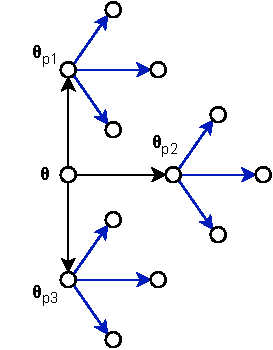
\includegraphics{figures/options.pdf}
    \caption[Visualization of two levels of options]
    {Visualization of a potential setup of 
    two levels of options.
    Black and blue arrows show 
    first-level and second-level options respectively. 
    $K$ perturbations are applied on each option on the 
    second level and $\bm{\theta}$ is updated to 
    either $\bm{\theta}_{p1}$,
    $\bm{\theta}_{p2}$ or $\bm{\theta}_{p3}$
    depending on which
    first-level option is the parent of the 
    best perturbation.
    }
    \label{figure:optionstree}
\end{figure}

\autoref{algorithm:options} gives the formal definition
of the method. 
Intuitively, the proposed method describes 
a lookahead into 
potential future updates from each point to select 
parameter updates 
which provide a continuous loss decrease 
over multiple steps.
An update is selected if one of its updates 
at the $\ell$-th level
gives the best objective. 
We hypothesize this will reduce the noise of
updates.

We remark that the type of lookahead we develop is in 
essence only slightly different to applying 
\autoref{algorithm:main} with larger batch sizes: When 
performing a single parameter update,
\autoref{algorithm:options} considers 
not only multiple mini-batches but also multiple
perturbations on the original parameter. We can say 
with batch size $b$, 
$(\ell+1) \cdot b$
samples and $\sum_{i=0}^\ell m^i \cdot K$ perturbations 
influence a parameter update, while each 
perturbation considers $b$ samples and from each point we 
have $K$ perturbations. We can look ahead to points up to 
$(\ell+1) \cdot R$ optimization steps away from the original parameter 
but each perturbation is still in the interval $[r, R]$.
Using options significantly increases the number 
of forward passes performed in each iteration with
$m^\ell \cdot K$ forward passes per tensor 
instead of only $K$. However, unlike using a larger 
batch size, any improvement in 
performance comes at no additional memory cost.  

\begin{algorithm} 
    \caption{\acl{GLD} Training with Options}
    \label{algorithm:options}
    \begin{algorithmic}[1]
        \For{$t=1, \dots, T$}
        % \State $x, y \gets$ \Call{GetMinibatch}{}
        \ForAll{tensor $\bm{\theta}_t$}
        % \State $\bm{\theta}_{t, \textrm{train}} \gets$ \Call{PickParametersToPerturb}{$\bm{\theta}_t$}
        % \ForAll{$p \in \psi(\bm{\theta}_t)$}
        % \State $\mathcal{J}(\bm{\theta}_{t, p}) \gets $ \Call{ComputeOptionLoss}{$\bm{\theta}_t$, $p$}
        % \EndFor
        \State $\mathbf{i} \gets $ \Call{SelectPerturbationIndices}{$\bm{\theta}_t$, $s$}
        \State $p^* \gets \arg \min_{p \in \psi(\bm{\theta}_t)} \{$\Call{ComputeOptionLoss}{$\bm{\theta}_t$, $p$, $\mathbf{i}$}$\}$ 
        \Comment{Best first-level option}
        \State $\bm{\theta}_{t+1} \gets \bm{\theta}_{t,p^*}$ 
        \State $\psi(\bm{\theta}_{t+1}) \gets \psi(p^*)$
        \EndFor
        \EndFor
        \Procedure{ComputeOptionLoss}{$\bm{\theta}_t$, $p$, $\mathbf{i}$}
        % \State $\bm{\theta}_{t,p} \gets$\Call{ApplyOption}{$\bm{\theta}_t$, $p$}
        \If{$\psi(p) = \emptyset$}
        \LComment{If this is the last level of options, apply perturbations to set the next level and return the minimum loss}
        \For {$k=1, \dots, K$}
        \State $r_k \gets 2^{-k}R(\bm{\theta}_t)$
        \State $\mathbf{v}_k \sim r_k \mathcal{D}$
        \State $\bm{\theta}_{t,p,k} \gets \bm{\theta}_{t,p}$
        \State $\bm{\theta}_{t,p,k}(\mathbf{i}) \gets \bm{\theta}_{t,p,k}(\mathbf{i}) + \mathbf{v}_k$ 
        \EndFor
        % \State $\mathcal{J} \gets \min_k\{\mathcal{J}(\bm{\theta}; x, y) | \bm{\theta} = \bm{\theta}_{t, \textrm{perturb}} , \bm{\theta} = \bm{\theta}_{t, \textrm{perturb}} + v_k\}$
        \State $\psi(p) \gets \arg\min_{p'}^{(m)}\{\mathcal{J}(\bm{\theta}_{t,p,p'}) \mid p' \in \{(\mathbf{i}, \mathbf{0}), (\mathbf{i}, \mathbf{v}_k) \mid k = 1, \dots K\}\}$
        \Comment{The top $m$ candidates}
        \State \Return $\min_k\{\mathcal{J}(\bm{\theta}_{t,p}), \mathcal{J}(\bm{\theta}_{t,p,k})\}$
        \Else
        \LComment{If this is not the last level of options, recursively return the minimum loss across all children}
        \State \Return $\min_{p' \in \psi(p)}\{$\Call{ComputeOptionLoss}{$\bm{\theta}_{t,p}$, $p'$, $\mathbf{i}$}$\}$
        % \State $\mathcal{J} \gets \infty$
        % \ForAll{child $p'$}
        % \State $\mathcal{J} \gets \min_{p' \in \textrm{children}(p)}\{\mathcal{J},$ \Call{ComputeOptionLoss}{$
        % _{t,p}$, $p'$}$\}$
        % \EndFor
        \EndIf
        % \State \Return $\mathcal{J}$
        \EndProcedure
    \end{algorithmic}
\end{algorithm}

% \section{Accelerated Forward Passes}
% Unlike first-order methods, our algorithm requires 
% multiple forward passes per iteration to update 
% parameters. To speed up the process,  
% \section{Weight Decay}

% \section{Implementation Details}
% % fast forward
% % give k instead of r, constant k 
\chapter{Experiments \& Results}
We test our methods on a binary classification task
provided by the SST-2 dataset \parencite{sst2}. 
The dataset consists of
sentences and smaller groups of words
extracted from movie reviews and 
human annotations of their sentiment as either 
positive (1) or negative (0). \autoref{table: sst2} 
shows some example input-output pairs. 

As our base model we use DistilBERT \parencite{distilbert},
which is a transformer model that 
uses knowledge distillation to reduce the size of a 
BERT model. The model consists of an embedding layer 
and 6 transformer layers with a hidden size of 768. 
For the binary classification task, a classification head
is attached to the base model, which is a fully-connected
feed-forward network consisting of a hidden layer of 
size 768 with \ac{ReLU} activation 
and an output layer of size 2. For our experiments we 
train only this classification head, which means we 
optimize 4 tensors: 
\begin{equation*}
    \mathbf{W}_1 \in \mathbb{R}^{768\times768};\quad 
    \mathbf{b}_1 \in \mathbb{R}^{1\times768};\quad 
    \mathbf{W}_2 \in \mathbb{R}^{768\times2};\quad 
    \mathbf{b}_2 \in \mathbb{R}^{1\times2}
\end{equation*}
Unless explicitly stated otherwise, we train all 
parameters of $\mathbf{b}_1, \mathbf{W}_2$ and 
$\mathbf{b}_2$, and randomly 
select $768\times2=1536$ parameters 
from $\mathbf{W}_1$ to perturb per iteration. 

Since we train only the classification head and not the
base model, we configure forward passes to calculate 
the output of the base model only once per iteration. 
This output is stored and further forward passes 
required by the algorithm in the same iteration 
calculate only the pass through the classification head,
improving the speed of computation.
% Later, we extend our experiments to use RoBERTa-large
% \parencite{roberta} as the base model. The classification head
% of this larger model has the same two-layer 
% structure but with a hidden size of 1024.  

We use \autoref{algorithm:options} for all experiments.
When an experiment does not involve options, we set 
both the number of option
levels $\ell$ and the number of options per level $m$ 
to 1, making it the equivalent of \autoref{algorithm:main}.
To ensure reproducibility, experiments set all 
random seeds to $42$. 

\begin{table}
    \centering
    \caption{Example input-output pairs from the SST-2 dataset}
    \label{table: sst2}
    \bigskip
    \begin{tabular}{l c}
        \toprule
        \textbf{Sentence} & \textbf{Label} \\
        \midrule
        contains no wit , only labored gags & 0 \\
        with his usual intelligence and subtlety  & 1\\
        we never feel anything for these characters & 0\\
        equals the original and in some ways even betters it & 1 \\
        \bottomrule
    \end{tabular}
\end{table}

\section{Hyperparameters}
There are several hyperparameters that can influence
the performance of \autoref{algorithm:main}. As discussed 
in \autoref{section:partitioning}, we define the search 
interval through a maximal radius $R$ and the number of 
searches per iteration $K$. Both $R$ and $K$ are 
hyperparameters as well as the batch size $b$.
Testing our main algorithm, we are interested in seeing 
how each of those hyperparameters affect performance.

\autoref{figure:r} shows validation 
accuracy for 3 of our experiments with different 
values for the maximal radius $R$
where we use the same $R$ for each of the 4 tensors.
As expected, the maximal radius $R$ is a deciding factor 
for the algorithm's performance. 
Generally, when $R$ is too low improvement is slow.
When it is too high, updates are noisy and the algorithm
fails to converge at a good minimum. 
We decide that $R=5\cdot10^{-3}$ is an adequate 
default value. 

The number of searches per iteration $K$ decides the 
size of the search interval. We expect better performance
with bigger intervals. The results shown in 
\autoref{figure:k} confirm this for 
small $K$. However, there are diminishing returns as 
$K$ grows.
% Conveniently, with only 1 search radius 
% we are able to get reasonable accuracy. 
Conveniently, the run with only one search radius per
iteration is able to get reasonable accuracy on 
our dataset. We remark that this might 
not be representative in general.
We note that for $K=1$, parameter updates behave like a 
stochastic two points update, 
where the algorithm decides whether the parameter should be 
updated with the given perturbation of radius $R$ or not. 
In particular, there is no binary search.

\begin{figure}
    \centering
    \begin{tikzpicture}
        \begin{axis}[
            width=0.8\textwidth,
            height=\axisdefaultheight,
            xlabel = {Iterations ($10^3$)},
            ylabel = {Accuracy},
            ymin = 71, ymax = 85, 
            xmin = 0, xmax = 40,
            xtick = {5, 10, 15, 20, 25, 30, 35, 40},
            ytick = {72, 74, 76, 78, 80, 82, 84},
            ymajorgrids = true,
            yminorgrids = true,
            legend pos = south east,
            grid style = dashed
        ]
        \addplot[color=blue, mark=square]
            coordinates {(0,0)(5, 51.03)(10,75.46)(15, 78.90)(20, 79.13)(25, 80.05)(30, 79.70)(35, 79.81)(40, 79.93)};
            \addlegendentry{$r_{\textrm{max}} = 2.5\cdot10^{-3}$}
    
        \addplot[color=orange, mark=square]
            coordinates {(0,0)(5, 53.33)(10,79.70)(15,80.50)(20, 80.62)(25, 80.96)(30, 78.90)(35, 81.19)(40, 82.11)};
            \addlegendentry{$r_{\textrm{max}} = 5\cdot10^{-3}$}
        
        \addplot[color=red, mark=square]
            coordinates {(0,0)(5, 59.52)(10,80.85)(15,80.50)(20, 79.47)(25, 77.98)(30, 78.67)(35, 79.47)(40, 77.29)};
            \addlegendentry{$r_{\textrm{max}} = 1\cdot10^{-2}$}    
    
        \end{axis}
    \end{tikzpicture}
    \caption[Validation Accuracy with different maximal search radii]
    {Validation Accuracy for three different values of maximal search radius.  
    $K$ is set to 5, batch size is 64.}
    \label{figure:r}
\end{figure}

\begin{figure}
    \centering
    \begin{tikzpicture}
        \begin{axis}[
            width=0.8\textwidth,
            height=\axisdefaultheight,
            xlabel = {Iterations ($10^3$)},
            ylabel = {Accuracy},
            ymin = 71, ymax = 85, 
            xmin = 0, xmax = 40,
            xtick = {5, 10, 15, 20, 25, 30, 35, 40},
            ytick = {72, 74, 76, 78, 80, 82, 84},
            ymajorgrids = true,
            yminorgrids = true,
            legend pos = south east,
            grid style = dashed
        ]
        \addplot[color=blue, mark=square]
            coordinates {(0,0)(5, 49.31)(10,76.83)(15,79.24)(20, 78.44)(25, 77.87)(30, 78.78)(35, 78.21)(40, 78.90)};
            \addlegendentry{$K=1$}
    
        \addplot[color=orange, mark=square]
            coordinates {(0,0)(5, 53.33)(10,79.70)(15,80.50)(20, 80.62)(25, 80.96)(30, 78.90)(35, 81.19)(40, 82.11)};
            \addlegendentry{$K=5$}
    
        \addplot[color=red, mark=square]
            coordinates {(0,0)(5, 48.51)(10,77.64)(15,80.73)(20, 80.16)(25, 80.73)(30, 80.50)(35, 81.54)(40, 80.05)};
            \addlegendentry{$K=9$}
        \end{axis}
    \end{tikzpicture}
    \caption[Validation Accuracy with different number
    of searches]
    {Validation Accuracy when performing
    1, 5 and 9 searches per iteration
    with maximal radius $R=5\cdot10^{-3}$. 
    Batch size is 64.}
    \label{figure:k}
\end{figure}

The batch size $b$ has the most significant effect on 
performance. \autoref{figure:b} shows 
validation accuracy with 3 different batch sizes.
We find that larger batch sizes perform 
consistently better. The drawback is a higher memory 
and time consumption with constant 
step count. We find the results with $b=64$ to be 
adequate and therefore conduct most of our experiments
with a batch size of 64.


\begin{figure}
    \centering
    \begin{tikzpicture}
        \begin{axis}[
            width=0.8\textwidth,
            height=\axisdefaultheight,
            xlabel = {Iterations ($10^3$)},
            ylabel = {Accuracy},
            ymin = 71, ymax = 85, 
            xmin = 0, xmax = 40,
            xtick = {5, 10, 15, 20, 25, 30, 35, 40},
            ytick = {72, 74, 76, 78, 80, 82, 84},
            ymajorgrids = true,
            yminorgrids = true,
            legend pos = south east,
            grid style = dashed
        ]
        \addplot[color=blue, mark=square]
            coordinates {(0,0)(5, 48.97)(10,75.92)(15,76.15)(20, 78.21)(25, 77.78)(30, 76.72)(35, 76.72)(40, 76.95)};
            \addlegendentry{$b = 16$}
    
        \addplot[color=orange, mark=square]
            coordinates {(0,0)(5, 53.33)(10,79.70)(15,80.50)(20, 80.62)(25, 80.96)(30, 78.90)(35, 81.19)(40, 82.11)};
            \addlegendentry{$b = 64$}
    
        \addplot[color=red, mark=square]
            coordinates {(0,0)(5, 52.29)(10,79.70)(15,81.31)(20, 81.54)(25, 81.42)(30, 82.80)(35, 82.57)(40, 84.17)};
            \addlegendentry{$b = 256$}
        \end{axis}
    \end{tikzpicture}
    \caption[Validation Accuracy with different batch sizes]
    {Validation Accuracy with 3 different batch sizes.
    $K$ is set to 5, $R$ is set to $5\cdot10^{-3}$.}
    \label{figure:b}
\end{figure}

Since they provide a suitable balance between performance,
memory and time consumption, we decide to take 
$R=5\cdot10^{-3}$, $K = 5$ and $b=64$ as
the set of hyperparameters we use when 
testing our other approaches and modifications over 
the base algorithm. In the following, we refer to this 
configuration as "default hyperparameters". 

% \begin{figure}
%     \centering
%     \begin{tikzpicture}
%         \begin{axis}[
%             width=0.8\textwidth,
%             height=\axisdefaultheight,
%             xlabel = {Iterations ($10^3$)},
%             ylabel = {Accuracy},
%             ymin = 0.35, ymax = 0.75, 
%             xmin = 0, xmax = 40,
%             xtick = {5, 10, 15, 20, 25, 30, 35, 40},
%             ytick = {0.4, 0.45, 0.5, 0.55, 0.6, 0.65, 0.7},
%             ymajorgrids = true,
%             yminorgrids = true,
%             legend pos = north east,
%             grid style = dashed
%         ]
%         \addplot[color=blue, mark=square]
%             coordinates {(0,1)(5, 0.6988)(10,0.5336)(15, 0.4618)(20, 0.4291)(25, 0.4125)(30, 0.404)(35, 0.3965)(40, 0.3897)};
%             \addlegendentry{$R = 2.5\cdot10^{-3}$}
    
%         \addplot[color=orange, mark=square]
%             coordinates {(0,1)(5, 0.7539)(10,0.4548)(15,0.4108)(20, 0.4073)(25, 0.3964)(30, 0.4014)(35, 0.3959)(40, 0.3945)};
%             \addlegendentry{$R = 5\cdot10^{-3}$}
        
%         \addplot[color=red, mark=square]
%             coordinates {(0,1)(5, 1.059)(10,0.4164)(15,0.4193)(20, 0.4304)(25, 0.4524)(30, 0.4569)(35, 0.493)(40, 0.4858)};
%             \addlegendentry{$R = 1\cdot10^{-2}$}    
    
%         \end{axis}
%     \end{tikzpicture}
%     \caption[Validation Accuracy for 3 different values of $R$]
%     {Validation Accuracy for 3 different values of $R$.  
%     $K$ is set to 5, batch size is 64.}
%     \label{figure:rtrain}
% \end{figure}

\section{Parameter Partitioning Methods} \label{section:partition}
In \autoref{section:partitioning}, we introduced 3 methods
to partition tensors that are too large 
to be trained efficiently by \ac{GLD}: We either sample
random indices or rank parameters based on absolute value 
or Fisher information estimate. The absolute value
and Fisher methods aim to select the most important 
parameters to train, improving the convergence rate as
the algorithm does not spend time on training unimportant
parameters with little effect on the outcome. 
From the four tensors we are training, 
% $\mathbf{W}_2, \mathbf{b}_1$ and $\mathbf{b}_2$ 
% have at most $768\times2$ parameters.  
$\mathbf{W}_1$ is the largest with size $768\times768$, 
followed by $\mathbf{W}_1$ with size $768\times2$.
We find that our algorithm can reliably train 
$768\times2$ parameters at a time, but $768\times768$ 
is too large. Therefore, we choose to select and train 
only $768\times2$
parameters from $\mathbf{W}_1$ per iteration. 
\autoref{figure:partition} shows validation loss
when training all parameters of $\mathbf{W}_1$ and when 
selecting $768\times2$ parameters randomly, through 
absolute value and through Fisher information estimate. 
$\mathbf{b}_1, \mathbf{W}_2$ and $\mathbf{b}_2$ each 
train all of their parameters. 
For the Fisher method we get a new Fisher information 
estimate every 10,000 steps. 
The algorithm diverges when training all $768\times768$
parameters of $\mathbf{W}_1$ using the default maximal 
radius. 
We find that contrary to our expectations, the importance 
methods do not bring an improvement on the rate of 
convergence. The performance of the absolute value method is 
comparable to that of the random method while the Fisher method 
performs worse. 
% We surmise that since the random method 
% does not discriminate based on some importance metric, 
% it trains all parameters more consistently, which ends
% up being beneficial for training with the given 
% configuration.

\begin{figure}
    \centering
    \begin{tikzpicture}
        \begin{axis}[
            width=0.8\textwidth,
            height=\axisdefaultheight,
            xlabel = {Iterations ($10^3$)},
            ylabel = {Loss},
            ymin = 0.40, ymax = 0.9, 
            xmin = 0, xmax = 40,
            xtick = {5, 10, 15, 20, 25, 30, 35, 40},
            ytick = {0.45, 0.50, 0.55, 0.60, 0.65, 0.7, 0.75, 0.8, 0.85},
            ymajorgrids = true,
            yminorgrids = true,
            legend pos = north east,
            grid style = dashed
        ]
        \addplot[color=black, mark=square]
            coordinates {(0,1)(5, 1.255)(10,0.5303)(15,0.7723)(20, 0.8727)(25, 1.01)(30, 1.091)(35, 1.139)(40, 1.388)};
            \addlegendentry{All}

        \addplot[color=blue, mark=square]
            coordinates {(0,1)(5, 0.6932)(10,0.471)(15,0.4386)(20, 0.4375)(25, 0.4308)(30, 0.4368)(35, 0.4278)(40, 0.4239)};
            \addlegendentry{Random}
    
        \addplot[color=orange, mark=square]
            coordinates {(0,1)(5, 0.6944)(10,0.4800)(15,0.4419)(20, 0.4355)(25, 0.4378)(30, 0.4498)(35, 0.4184)(40, 0.4427)};
            \addlegendentry{Absolute value}
    
        \addplot[color=red, mark=square]
            coordinates {(0,1)(5, 0.7134)(10,0.4741)(15,0.4563)(20, 0.4728)(25, 0.4436)(30, 0.4444)(35, 0.4802)(40, 0.4520)};
            \addlegendentry{Fisher}
        \end{axis}
    \end{tikzpicture}
    \caption[Validation loss with different parameter partitioning methods]
    {Validation loss of different parameter partitioning methods on 
    $\mathbf{W}_1$ using default hyperparameters. Other tensors are not split.}
    \label{figure:partition}
\end{figure}

% \begin{figure}
%     \centering
%     \begin{tikzpicture}
%         \begin{axis}[
%             width=0.8\textwidth,
%             height=\axisdefaultheight,
%             xlabel = {Iterations ($10^3$)},
%             ylabel = {Accuracy},
%             ymin = 71, ymax = 85, 
%             xmin = 0, xmax = 40,
%             xtick = {5, 10, 15, 20, 25, 30, 35, 40},
%             ytick = {72, 74, 76, 78, 80, 82, 84},
%             ymajorgrids = true,
%             yminorgrids = true,
%             legend pos = south east,
%             grid style = dashed
%         ]
%         \addplot[color=blue, mark=square]
%             coordinates {(0,0)(5, 51.72)(10,78.9)(15,80.05)(20, 80.50)(25, 79.7)(30, 79.7)(35, 81.08)(40, 79.82)};
%             \addlegendentry{Absolute value}
    
%         \addplot[color=orange, mark=square]
%             coordinates {(0,0)(5, 53.33)(10,79.70)(15,80.50)(20, 80.62)(25, 80.96)(30, 78.90)(35, 81.19)(40, 82.11)};
%             \addlegendentry{Random}
    
%         \addplot[color=red, mark=square]
%             coordinates {(0,0)(5, 50.92)(10,78.9)(15,79.24)(20, 78.33)(25, 78.33)(30, 79.36)(35, 75.23)(40, 78.67)};
%             \addlegendentry{Fisher}
%         \end{axis}
%     \end{tikzpicture}
%     \caption[Partition]
%     {Partition}
%     \label{figure:partitionacc}
% \end{figure}

\section{Radius Scheduling} \label{section:schedule}
We introduce a radius scheduler to each of the trainable 
tensors that reduces the maximum search radius 
as training goes on. We use a linear schedule $s$ that scales 
from 1 to $h = 0.1$ over the course of training $T$ steps:
\begin{equation}
    s(t) = 1 - \frac{t(1-h)}{T}                                                                                                                                                                                                                                                                                                                                                                                                                                                                                                                                                                                                                                                                                                                                                                                                                                                                                                                                                                                                                                                                                                                                                                                                                                                                                                                                                                                                                                                                                                                                                                                                                                                                                                                                                                                                                                                                                                                                                                                                                                                                                                                                                                                                                                                                                                                                                                                                                                                             
\end{equation}
Maximal radius at step $t$ is calculated by 
multiplying the 
maximal radius of the tensor with the schedule:
\begin{equation}
    R(\bm{\theta}_t) = R(\bm{\theta}) \cdot s(t)
\end{equation}
We use the same schedule with all parameters as well as 
the same initial maximal radius. \autoref{figure:schedule}
shows the validation loss for this experiment in comparison
to the original result with no schedule. 
We find that 
without the radius schedule the model learns faster 
initially but overall loss is less stable and 
the radius scheduler outperforms at later steps. 
Still, a confident increase in performance is not 
observed with default hyperparameters. 
One of our hypotheses was that using a radius scheduler,
the algorithm could retain its convergence with 
fewer searches. To test this, 
We redo the experiment with $K=1$. The results are shown in 
\autoref{figure:schedule2}.
We observe that the effect of the radius scheduler 
is amplified when doing only one search per iteration.
In particular, it causes loss to more consistently decrease 
throughout the entire duration of training. 
While $K=5$ still performs better, the gap is significantly
smaller. We surmise that a smaller $K$ could be used in 
conjunction with a radius scheduler when an increase in 
computation speed is desired.


\begin{figure}
    \centering
    \begin{tikzpicture}
        \begin{axis}[
            width=0.8\textwidth,
            height=\axisdefaultheight,
            xlabel = {Iterations ($10^3$)},
            ylabel = {Loss},
            ymin = 0.40, ymax = 0.49, 
            xmin = 0, xmax = 80,
            xtick = {10, 20, 30, 40, 50, 60, 70, 80},
            ytick = {0.41, 0.42, 0.43, 0.44, 0.45, 0.46, 0.47, 0.48},
            ymajorgrids = true,
            yminorgrids = true,
            legend pos = north east,
            grid style = dashed
        ]
        \addplot[color=blue, mark=square]
            coordinates {(0,1)(10,0.471)(20, 0.4375)(30, 0.4368)(40, 0.4239)(50, 0.4363)(60, 0.4364)(70, 0.4439)(80, 0.4604)};
            \addlegendentry{No schedule ($K=5$)}
    
        \addplot[color=red, mark=square]
            coordinates {(0,1)(10,0.4863)(20, 0.4536)(30, 0.4416)(40,0.434)(50,0.4376)(60,0.4301)(70, 0.4274)(80, 0.4261)};
            \addlegendentry{Linear schedule ($K=5$)}
        \end{axis}
    \end{tikzpicture}
    \caption[Validation loss with and without a radius scheduler]
    {Validation loss with and without a linear radius 
    scheduler using default hyperparameters}
    \label{figure:schedule}
\end{figure}

\begin{figure}
    \centering
    \begin{tikzpicture}
        \begin{axis}[
            width=0.8\textwidth,
            height=\axisdefaultheight,
            xlabel = {Iterations ($10^3$)},
            ylabel = {Loss},
            ymin = 0.40, ymax = 0.49, 
            xmin = 0, xmax = 80,
            xtick = {10, 20, 30, 40, 50, 60, 70, 80},
            ytick = {0.41, 0.42, 0.43, 0.44, 0.45, 0.46, 0.47, 0.48},
            ymajorgrids = true,
            yminorgrids = true,
            legend pos = south west,
            grid style = dashed
        ]
        \addplot[color=blue, mark=square]
            coordinates {(0,1)(10, 0.5058)
            (20,0.4833)(30,0.4673)
            (40, 0.4586)(50, 0.484)
            (60, 0.4899)(70, 0.495)
            (80, 0.4924)};
            \addlegendentry{No schedule ($K=1$)}

        \addplot[color=red, mark=square]
            coordinates {(0,1)
            (10,0.5313)
            (20, 0.4672)
            (30, 0.4529)
            (40,0.4492)
            (50,0.4497)
            (60,0.4459)
            (70, 0.4315)
            (80, 0.4333)};
            \addlegendentry{Linear schedule ($K=1$)}
        \end{axis}
    \end{tikzpicture}
    \caption[Validation loss with and without a radius scheduler with only one search per iteration]
    {Validation loss with and without a linear radius 
    scheduler when performing only one search per iteration}
    \label{figure:schedule2}
\end{figure}

\section{Weight Decay}
We investigate the effects of adding an $L_2$-regularizer 
to the objective function:
\begin{equation}
    \mathcal{J}(\bm{\theta}) = \mathcal{L}(\bm{\theta}) + \lambda \cdot \Vert \bm{\theta} \Vert_2
\end{equation}
where $\mathcal{L}$ is the cross-entropy loss and 
$\lambda$ is the norm weight. 
\autoref{figure:decay} compares three different values
of $\lambda$. Our original experiment without weight decay
has $\lambda = 0$. We observe a more stable decrease in 
loss with regularization. The hyperparameter $\lambda$ 
plays a crucial role in the effectiveness of this method 
as it controls the balance between regularization
and error minimization. We consider
$\lambda = 0.05$ to be a good default value. 

\begin{figure}
    \centering
    \begin{tikzpicture}
        \begin{axis}[
            width=0.8\textwidth,
            height=\axisdefaultheight,
            xlabel = {Iterations ($10^3$)},
            ylabel = {Loss},
            ymin = 0.40, ymax = 0.49, 
            xmin = 0, xmax = 80,
            xtick = {10, 20, 30, 40, 50, 60, 70, 80},
            ytick = {0.41, 0.42, 0.43, 0.44, 0.45, 0.46, 0.47, 0.48},
            ymajorgrids = true,
            yminorgrids = true,
            legend pos = north east,
            grid style = dashed
        ]
        \addplot[color=blue, mark=square]
            coordinates {(0,0.7)(10,0.471)(20, 0.4375)(30, 0.4368)(40, 0.4239)(50, 0.4363)(60, 0.4364)(70, 0.4439)(80, 0.4604)};
            \addlegendentry{$\lambda = 0$}
    
        \addplot[color=orange, mark=square]
            coordinates {(0,0.7)
            (10, 0.5155)
            (20, 0.4632)
            (30, 0.4366)
            (40, 0.4293)
            (50, 0.4349)
            (60, 0.4241)
            (70, 0.4146)
            (80, 0.4166)};
            \addlegendentry{$\lambda = 0.05$}

        \addplot[color=red, mark=square]
            coordinates {(0,0.7)
            (10, 0.5435)
            (20, 0.4961)
            (30, 0.469)
            (40, 0.4565)
            (50, 0.4554)
            (60, 0.4377)
            (70, 0.4352)
            (80, 0.4292)};
            \addlegendentry{$\lambda = 0.1$}
        \end{axis}
    \end{tikzpicture}
    \caption[Validation loss using weight decay with different norm weights]
    {Validation loss using weight decay with different norm weights.}
    \label{figure:decay}
\end{figure}


\section{Options}
\autoref{algorithm:options} introduces 2 additional 
hyperparameters: The number of option levels $\ell$ and
the number of options per level $m$. Both hyperparameters
have a significant effect on 
the time requirement of the algorithm: The number of 
forward passes each iteration is $n \cdot m^\ell \cdot K$ 
when training $n$ tensors. Therefore, 
although we anticipate a reduction in update noise 
when using options, we have to pick $\ell$ and $m$ 
conservatively in order to keep within a reasonable 
computation time. \autoref{figure:options} shows validation 
loss for four experiments with different values of 
$m$ and $\ell$, each of them named $m \times \ell$.
We observe moderate improvements in loss as $m \times \ell$
increases with $\ell$ having a larger effect than $m$. 

\begin{figure}
    \centering
    \begin{tikzpicture}
        \begin{axis}[
            width=0.8\textwidth,
            height=\axisdefaultheight,
            xlabel = {Iterations ($10^3$)},
            ylabel = {Loss},
            ymin = 0.40, ymax = 0.49, 
            xmin = 0, xmax = 80,
            xtick = {10, 20, 30, 40, 50, 60, 70, 80},
            ytick = {0.41, 0.42, 0.43, 0.44, 0.45, 0.46, 0.47, 0.48},
            ymajorgrids = true,
            yminorgrids = true,
            legend pos = north east,
            grid style = dashed
        ]
        \addplot[color=blue, mark=square]
            coordinates {(0,1)(10,0.471)(20, 0.4375)(30, 0.4368)(40, 0.4239)(50, 0.4363)(60, 0.4364)(70, 0.4439)(80, 0.4604)};
            \addlegendentry{$1\times1$}

        \addplot[color=green!60!black, mark=square]
            coordinates { (0,1)
            (10, 0.4795)
            (20, 0.4403)
            (30, 0.4327)
            (40, 0.4167)
            (50, 0.4322)
            (60, 0.4183)
            (70, 0.4377)
            (80, 0.4421)
            }; \addlegendentry{$3\times1$}        
    
        \addplot[color=orange, mark=square]
            coordinates { (0,1)
            (10, 0.4821)
            (20, 0.4284)
            (30, 0.4232)
            (40, 0.4066)
            (50, 0.4251)
            (60, 0.4216)
            (70, 0.4197)
            (80, 0.4296)
            }; \addlegendentry{$2\times2$}
        \addplot[color=red, mark=square]
            coordinates {(0,1)(10, 0.4744)(20, 0.4269)(30, 0.4137)(40, 0.4161)(50, 0.4143)(60, 0.4213)(70, 0.4108)(80, 0.4157)};
            \addlegendentry{$3\times2$}
        \end{axis}
    \end{tikzpicture}
    \caption[Validation loss for different values of option width and depth]
    {Validation loss for different values of option width and depth.
    We refer to $m$ options per level with $\ell$ levels as $m \times \ell$.}
    \label{figure:options}
\end{figure}

\section{Final Results \& Preferred Method}
To test the interoperability of our methods, we perform 
an experiment using both radius scheduling and 
weight decay at the same time. 
\autoref{figure:final} shows the validation loss 
for this experiment with and without using options.
\autoref{figure:final2} shows a repeat of this experiment
with an increased maximal radius of $R = 7.5 \cdot 10^{-3}$.
An experiment that uses this maximal radius 
without radius scheduling or weight decay is shown
for comparison. We find that using both a linear 
radius schedule and weight decay allows the use 
of higher maximal search radii for faster convergence. 
% We obtain our best results in terms of loss 
% with this configuration. 
This configuration yields our best results in terms
of loss and thus becomes our preferred method. We find 
that the effects of using options are 
negligible with this configuration and hence opt 
not to use them.  
\autoref{table:results} compares our methods in terms 
of validation accuracy and memory consumption with 
a state-of-the-art
Adam optimizer. We find that GLD uses slightly less memory 
than Adam. With a batch size of 64, GLD yields a slightly
lower accuracy than Adam, but the accuracy gap closes 
with a batch size of 256. 
% Although our preferred method 
% provides a significant loss improvement over 
% our default GLD method, this improvement 
% does not result in a noticeably higher accuracy 
% under this experiment configuration.

\begin{figure}
    \centering
    \begin{tikzpicture}
        \begin{axis}[
            width=0.8\textwidth,
            height=\axisdefaultheight,
            xlabel = {Iterations ($10^3$)},
            ylabel = {Loss},
            ymin = 0.40, ymax = 0.49, 
            xmin = 0, xmax = 80,
            xtick = {10, 20, 30, 40, 50, 60, 70, 80},
            ytick = {0.41, 0.42, 0.43, 0.44, 0.45, 0.46, 0.47, 0.48},
            ymajorgrids = true,
            yminorgrids = true,
            legend pos = north east,
            grid style = dashed
        ]
        \addplot[color=blue, mark=square]
            coordinates { (0,1)
            (10, 0.511)
            (20, 0.462)
            (30, 0.4527)
            (40, 0.4379)
            (50, 0.4272)
            (60, 0.4283)
            (70, 0.4279)
            (80, 0.4294)
            }; \addlegendentry{$1\times1$}        
    
        \addplot[color=red, mark=square]
            coordinates { (0,1)
            (10, 0.517)
            (20, 0.4665)
            (30, 0.4474)
            (40, 0.4431)
            (50, 0.435)
            (60, 0.4361)
            (70, 0.4366)
            (80, 0.4362)
            }; \addlegendentry{$3\times2$}
        \end{axis}
    \end{tikzpicture}
    \caption[Validation loss for two experiments applying both 
    a linear radius schedule and weight decay]
    {Validation loss for two experiments applying both 
    a linear radius schedule and weight decay with $\lambda = 0.05$ 
    using default hyperparameters.}
    \label{figure:final}
\end{figure}

\begin{figure}
    \centering
    \begin{tikzpicture}
        \begin{axis}[
            width=0.8\textwidth,
            height=\axisdefaultheight,
            xlabel = {Iterations ($10^3$)},
            ylabel = {Loss},
            ymin = 0.40, ymax = 0.49, 
            xmin = 0, xmax = 80,
            xtick = {10, 20, 30, 40, 50, 60, 70, 80},
            ytick = {0.41, 0.42, 0.43, 0.44, 0.45, 0.46, 0.47, 0.48},
            ymajorgrids = true,
            yminorgrids = true,
            legend pos = south west,
            grid style = dashed
        ]
        \addplot[color=blue, mark=square]
        coordinates { (0,1)
        (10, 0.4751)
        (20, 0.4455)
        (30, 0.4294)
        (40, 0.4239)
        (50, 0.4342)
        (60, 0.4306)
        (70, 0.4151)
        (80, 0.4157)
        }; \addlegendentry{$1\times1$}        

    \addplot[color=red, mark=square]
        coordinates { (0,1)
        (10, 0.4842)
        (20, 0.4382)
        (30, 0.429)
        (40, 0.4247)
        (50, 0.424)
        (60, 0.418)
        (70, 0.4252)
        (80, 0.419)
        }; \addlegendentry{$3\times2$}

    \addplot[color=orange, mark=square]
        coordinates { (0,1)
        (10, 0.4668)
        (20, 0.4504)
        (30, 0.4578)
        (40, 0.4837)
        (50, 0.484)
        (60, 0.4584)
        (70, 0.4892)
        (80, 0.4729)
        }; \addlegendentry{control}
        \end{axis}
    \end{tikzpicture}
    \caption[Validation loss for two experiments applying both 
    a linear radius schedule and weight decay with a higher maximal radius]
    {Validation loss for two experiments applying both 
    a linear radius schedule and weight decay with $\lambda = 0.05$ 
    using a maximal radius of $R = 7.5 \cdot 10^{-3}$.
    The third control experiment uses the same $R$ but does not use
    a radius scheduler or weight decay.}
    \label{figure:final2}
\end{figure}

\begin{table}
    \centering
    \caption [Comparison of GLD and Adam in terms of 
    validation accuracy on SST-2 and memory consumption]
    {Comparison of GLD and Adam in terms of 
    validation accuracy on SST-2 and memory consumption.
    The Adam optimizer
    uses a learning rate of $5 \cdot 10^{-5}$ and a linear
    learning rate schedule. GLD methods set $K=5$ and
    $R = 5 \cdot 10^{-3}$. GLD* refers to our preferred 
    method, setting $R = 7.5 \cdot 10^{-3}$ while
    applying a linear radius schedule and 
    weight decay with $\lambda = 0.05$.
    Experiments with batch size 64
    run for $80,000$ steps, those with batch size 256 
    run for $40,000$ steps. Validation accuracy is 
    computed every $5,000$ steps.
    }
    \label{table:results}
    \bigskip
    \begin{tabular}{c c c c}
        \toprule
        \textbf{Optimizer} & \textbf{Batch Size} & \textbf{Validation Accuracy} & \textbf{Memory Consumption} \\
        \midrule
        GLD & 64 & 82.11\% & 409 MiB \\
        GLD* & 64 & 82.22\% & 409 MiB \\
        GLD & 256 & 84.17\% & 854 MiB \\
        Adam & 64 & 84.75\% & 421 MiB \\
        Adam & 256 & 84.40\% & 867 MiB \\
        \bottomrule
    \end{tabular}
\end{table}


\chapter{Discussion \& Future Work} \label{chapter:discussion}
This chapter evaluates our approaches and suggests 
future research directions that arise from our work.
We will discuss the strengths and shortcomings 
of our methods, as well as possible modifications that 
might improve the effectiveness and experiments that might 
provide useful results. 
% Then, we will put forward
% new ideas that can improve the efficiency and reliability
% of direct search methods for language model fine-tuning.

Our experiments show that the effectiveness of our methods
depends largely on batch size where larger batch sizes 
consistently perform better. This outcome is hardly 
surprising as it has already been established for 
gradient methods that larger batch sizes result in better 
parameter updates by giving descent directions more
representative of the entire dataset, reducing the
probability of choosing parameters that give a worse 
overall representation.  We suspect that 
this effect might be amplified for direct search methods
since random parameter updates that do not make use of 
gradient information are also not necessarily in the 
optimal descent direction for a given batch. 
% by reducing the variance of the 
% gradient. While the effects are similar for 
% direct search methods, we suspect that
% the effect of batch size in reducing
% the probability of choosing parameters that give
% a worse representation of the dataset is amplified.
% Random parameter updates that do not make use of gradient
% information are not necessarily in the 
% optimal descent direction for a given batch. 
% we suspect that 
% the importance of batch size is amplified
% with random parameter updates to reduce the probability 
% of choosing updates that give a worse representation of 
% the whole dataset. 
% as random parameter updates that 
% do not make use of gradient information
% inherently have high variance. 
This might make it a necessity to 
pick a larger batch size than a first-order
method in order to be able to compete with it. 
This of course seems counter-productive considering our 
main objective of reducing memory consumption. However,
for larger networks, the memory gains from 
eliminating backpropagation can offset
the additional memory usage due to the larger batch size.
On the other hand, our experiments on the Adam optimizer
did not yield a better accuracy when we increased the 
batch size, which might indicate that for larger 
batch sizes, the performance of our method could 
be on the same level as that of first-order methods using the same 
batch size.
In any case, experimenting with larger batch sizes 
can provide valuable data.   

% While that outcome is 
% hardly surprising, we suspect that for stochastic 
% derivative-free methods the importance of 
% batch size is amplified and 
% It has already been established for gradient methods
% that larger batch sizes give better parameter updates
% as they reduce the variance of the gradient. 

Our method of partitioning parameters might not be
optimal. Since we first consider individual tensors
as a unit of training and only then 
further partition a unit if it is too large, 
our algorithms might spend excessive time 
on some parameters while seldom updating others.
For example, our algorithm considers the same number of 
perturbations for the $1\times2$ 
bias of the output layer
as the $768\times768$ weight matrix of the hidden layer,
of which only a smaller partition of size $s=768\times2$ 
is optimized in each step. 
A more clever way of splitting trainable parameters 
could gain efficiency in terms of convergence rate.
One could, for example, consider the entire set of 
trainable parameters as a single large unit and 
select $s$ indices at random from that large unit 
to train each step. 
While our original method stems from initial intuition 
and ease of implementation, it can also have the 
advantage of making sure all weights and biases of 
the network are trained in each step. 

The number of parameters $s$ we select to train from 
from the large weight matrix is decided empirically. 
It copies the size of the second largest weight matrix 
that we train, because we have seen through 
experimentation that a matrix of that size could be trained 
by our algorithm. 
It is known that direct search methods lose 
performance with larger parameter dimensions and our 
experiments in \autoref{section:partition} confirm 
that training the entire $768\times768$ matrix 
is not feasible with our algorithm. However,
there could be a better value 
for $s$. We expect that with smaller $s$, the algorithm
will still learn but with a slower convergence rate 
as fewer parameters are optimized each step. 
Conversely, larger values could provide faster 
convergence, but performance will suffer when $s$ is 
too large. Experimenting with both smaller and 
larger values of $s$ could lead to a better understanding
of the effects of dimensionality on the algorithm.

We designed the method of using options as a way to 
direct the algorithm towards parameter updates that 
give a better representation of the entire dataset
without increasing the batch size. Our experiments
indicate that using options improves loss with no
additional memory cost. However, there is a 
significant increase in time cost as the number
of forward passes increases. Whether or not options 
should be used depends therefore on time 
constraints. Using deeper levels of options 
could bring further improvement, however becomes 
less practical as time usage will be excessive 
compared to a similarly performing first-order method.
It could also be interesting to 
see how the performance gains are affected by batch size.
Since larger batch sizes are already more representative 
of the entire dataset, improvements brought 
by options might become less impactful.

We find that using the linear radius schedule we define in
\autoref{section:schedule} as well as weight decay, 
we achieve better results 
by increasing the initial radius. 
One could increase the minimal
multiplier $h$ of the scheduler for a flatter schedule where maximal
radius changes slower in a smaller interval 
throughout training. It could also be interesting to 
experiment 
with different types of schedule function such as cosine 
annealing \parencite{cosine} or to apply a warmup 
strategy \parencite{warmup}. 

One weakness of getting parameter updates 
solely through random perturbations is that 
previous update steps are not considered. 
Intuitively, an update direction that 
has improved the model in one training iteration 
should be more likely to improve it further 
than, for example, the exact opposite direction. 
Our algorithm, however, cannot
make use of this assumption and samples both 
directions with the same probability when searching for 
improving perturbations. 
A possible improvement is to implement a
system similar to momentum that factors in previous 
update directions when calculating random 
perturbations. 
Update candidates could then be computed by adding
a vector accumulating previous updates with some 
momentum coefficient to the random perturbation 
sampled from the original distribution, effectively
shifting the distribution towards the region of 
perturbation vectors that have 
previously improved the model. 
The amount of improvement an update brings could 
also be part of the formulation. We think that 
being able to select better candidates to consider
is an important step to optimizing the algorithm for time  
and that the described approach or a derivative thereof
can improve the convergence 
rate by making it more likely 
for a sampled candidate to be improving the model.

Introducing parallelism could be another way of 
optimizing the algorithm for time. The key factor
making the algorithm slow is the large number of forward
passes it requires. Each training step requires multiple
forward passes with the same batch. Computing  
those in separate processing units or 
threads of execution can speed up 
the algorithm significantly. 
% The forward passes of a training
% step could be computed 
% in separate processing units or threads of execution.

% It is 
% likely that an update direction that has improved the
% model in one training iteration, improves it further

  

% momentum like SMTP 
% fine tune base model (with K=1?)
% better gpu usage / parallelism
% even higher batch size experiment  

% options no memory but time - worth?
% scheduling - maybe with bigger max-r?, 
% more effective with / could allow smaller K.
% batch size - critical. more critical than with gradient?
% partitioning - could be more efficient. 
% training 2 parameters for bias.
% number of parameters to train completely empirical, 
% might not be ideal. 
\chapter{Conclusion}
We have introduced a recipe for training neural networks 
using an optimizer based on the \acf{GLD}
algorithm \parencite{gld}. 
Being a zeroth-order
optimization algorithm, \ac{GLD} does not 
make use of gradient information when updating 
parameters. This removes the 
need for a backward pass on the network, which can have 
a significant impact on memory consumption.
\ac{GLD} is a direct search method, which means that
unlike many state-of-the-art zeroth-order 
optimizers that have been used with neural networks, 
our method does not rely on an estimation of the 
gradient and instead selects parameter updates 
from a set of randomly sampled perturbations
of the parameter. 
We think that direct search methods have the potential
to create memory-efficient optimizers of neural 
networks, which motivates our work.

A known limitation of direct search methods is that 
their performance deteriorates as the number of variables 
increases \parencite{directsearch}. 
Our main contribution is introducing a parameter 
partitioning method to split the set of trainable 
parameters of the model into smaller subsets in order
to bypass this limitation. 
% in order to bypass a known limitation of direct 
% search methods, which is that their 
% performance deteriorates as the number of variables 
% increases \parencite{directsearch}. 
The size of the 
subsets is chosen empirically to be sufficiently small, such 
that \ac{GLD} is able to train an individual subset
with a reasonable rate of convergence.
% Training one subset at a time, we are then able to train 
% the entire network. 
We are then able to train the entire network by 
cycling through the subsets in each iteration, 
training one subset at a time. Our method takes each
individual weight matrix and bias vector as a subset, 
which is further divided if the size is too large
by selecting parameters either randomly or
based on importance, using the absolute value or
an estimation of the Fisher importance matrix
as the importance measure. 

We also propose additional modifications on the algorithm 
with the aim of  
further improving its performance.
We introduce radius scheduling, the application 
of a learning rate schedule onto the maximal
search radius of \ac{GLD}, and 
weight decay, which adds an $L_2$-norm regularizer 
to the objective function. Both methods are motivated 
by their established 
success in improving first-order methods and our 
experiments show that they are applicable 
for direct search methods as well. We introduce 
options, which is a method that implements 
a lookahead into potential future updates that are then
considered when choosing the current update. 
We apply options as a way to choose parameter updates 
that are more representative of the entire 
training dataset without increasing the batch size. 

To test our methods, we
fine-tune a classifier attached to a pre-trained
DistilBERT model for the binary 
classification task given by the SST-2 dataset. 
We obtain
our best results by using 
% a combination of our methods. 
both radius scheduling and weight decay on top of 
our main parameter partitioning method where we 
pick parameters at random when the weight matrix is 
too large. 
When compared to Adam, our method gives slightly reduced 
accuracy while using less memory. The difference in 
accuracy seems to decrease as batch size increases.
We identify the slow speed of our algorithm as 
a major drawback. We think that future 
work can both further close the accuracy gap to 
state-of-the-art first-order methods and 
speed up the algorithm, addressing this drawback.


% with a small reduction in accuracy
% compared to Adam, 
% a state-of-the-art first-order optimizer. 

% Eliminating the backward pass has a 
% significant positive impact on memory consumption. 
% TODO: add more chapters here

\appendix{}

\microtypesetup{protrusion=false}

\addchap{Abbreviations}
\begin{acronym}
	\itemsep-.25\baselineskip
	\acro{TUM}[TUM]{Technical University of Munich}
	\acro{NLP}{Natural Language Processing}
	\acro{tanh}{Hyperbolic Tangent}
	\acro{ReLU}{Rectified Linear Unit}
	\acro{SGD}{Stochastic Gradient Descent}
	\acro{SPSA}{Simultaneous Perturbation Stochastic Approximation}
	\acro{GLD}{Gradientless Descent}
	\acro{LLM}{Large Language Model}
	\acro{STP}{Stochastic Three Points}
	\acro{SMTP}{Stochastic Momentum Three Points}
	\acro{FIM}{Fisher Importance Matrix}
	\acro{RNN}{Recurrent Neural Network}
	% TODO: add acronyms
\end{acronym}

\listoffigures{}
\listoftables{}
\microtypesetup{protrusion=true}
\printbibliography{}

\end{document}
